%%%%%%%%%%%%%%%%%%%%%%%%%%%%%%%%%%%%%%%%%
% Classicthesis Typographic Thesis
% LaTeX Template
% Version 1.1 (4/8/12)
%
% This template has been downloaded from:
% http://www.LaTeXTemplates.com
%
% Original author:
% André Miede (http://www.miede.de)
%
% License:
% CC BY-NC-SA 3.0 (http://creativecommons.org/licenses/by-nc-sa/3.0/)
%
% General Tips:
% 1) Make sure to edit the classicthesis-config.file
% 2) New enumeration (A., B., C., etc in small caps): \begin{aenumerate} \end{aenumerate}
% 3) For margin notes: \marginpar or \graffito{}
% 4) Do not use bold fonts in this style, it is designed around them
% 5) Use tables as in the examples
% 6) See classicthesis-preamble.sty for useful commands
%
%%%%%%%%%%%%%%%%%%%%%%%%%%%%%%%%%%%%%%%%%

%------------------------------------------------
%	PACKAGES AND OTHER DOCUMENT CONFIGURATIONS
%------------------------------------------------

\documentclass[
	twoside,titlepage,numbers=noenddot,headinclude,%1headlines,
    footinclude=true,cleardoublepage=empty,
    BCOR=5mm,paper=a4,fontsize=11pt, % Binding correction, paper type and font size
    english, % Languages
]{scrreprt} 
                
% Includes the file which contains all the document configurations and packages - make sure to edit this file
%%%%%%%%%%%%%%%%%%%%%%%%%%%%%%%%%%%%%%%%%
% Thesis Configuration File
%
% The main lines to change in this file are in the DOCUMENT VARIABLES
% section, the rest of the file is for advanced configuration.
%
%%%%%%%%%%%%%%%%%%%%%%%%%%%%%%%%%%%%%%%%%

%----------------------------------------------------------------------------------------
%	DOCUMENT VARIABLES
%	Fill in the lines below to enter your information into the thesis template
%	Each of the commands can be cited anywhere in the thesis
%----------------------------------------------------------------------------------------

% Remove drafting to get rid of the '[ Date - classicthesis version 4.0 ]' text at the bottom of every page
\PassOptionsToPackage{eulerchapternumbers,listings,pdfspacing,subfig,beramono,eulermath,parts,dottedtoc,tocaligned}{classicthesis}
% Available options: drafting parts nochapters linedheaders eulerchapternumbers beramono eulermath pdfspacing minionprospacing tocaligned dottedtoc manychapters listings floatperchapter subfig
% Adding 'dottedtoc' will make page numbers in the table of contents flushed right with dots leading to them

\newcommand{\myTitle}{Tangible\xspace}
\newcommand{\mySubtitle}{A Python library to convert data into tangible 3D models.\xspace}
\newcommand{\myThesis}{Student Research Project Thesis\xspace}
\newcommand{\myName}{Danilo Bargen\xspace}
\newcommand{\myProf}{Prof. Dr. Josef M. Joller\xspace}
\newcommand{\myFaculty}{ITA Institute for Internet Technologies and Applications\xspace}
\newcommand{\myDepartment}{Department of Computer Science\xspace}
\newcommand{\myUni}{HSR University of Applied Science Rapperswil\xspace}
\newcommand{\myLocation}{Rapperswil\xspace}
\newcommand{\myTime}{Fall 2013\xspace}
\newcommand{\myVersion}{version 1.0\xspace}
\newcommand{\myLicense}{CC BY-SA 3.0 Unported\xspace}
\newcommand{\myKeywords}{3D Printing, CAD, Cross Compilers, Data Analysis, Data
Visualization, OpenSCAD, Python, Software Libraries, Statistics, Tangible}

%----------------------------------------------------------------------------------------
%	USEFUL COMMANDS
%----------------------------------------------------------------------------------------

\newcommand{\ie}{i.\,e.}
\newcommand{\Ie}{I.\,e.}
\newcommand{\eg}{e.\,g.}
\newcommand{\Eg}{E.\,g.} 

\newcommand{\tangible}{\emph{Tangible}}

\newcounter{dummy} % Necessary for correct hyperlinks (to index, bib, etc.)
\providecommand{\mLyX}{L\kern-.1667em\lower.25em\hbox{Y}\kern-.125emX\@}

%----------------------------------------------------------------------------------------
%	PACKAGES
%----------------------------------------------------------------------------------------

\usepackage{lipsum} % Used for inserting dummy 'Lorem ipsum' text into the template

%------------------------------------------------
 
\PassOptionsToPackage{utf8}{inputenc}
\usepackage{inputenc}
 
%------------------------------------------------

\PassOptionsToPackage{american}{babel}
\usepackage{babel}

%------------------------------------------------			

\PassOptionsToPackage{square,numbers}{natbib}
\usepackage{natbib}
 
%------------------------------------------------

\PassOptionsToPackage{fleqn}{amsmath} % Math environments and more by the AMS 
\usepackage{amsmath}
 
%------------------------------------------------

\PassOptionsToPackage{T1}{fontenc}
\usepackage{fontenc}

%------------------------------------------------

\usepackage{xspace} % To get the spacing after macros right

%------------------------------------------------

\usepackage{mparhack} % To get marginpar right

%------------------------------------------------

\usepackage{fixltx2e} % Fixes some LaTeX stuff 

%------------------------------------------------

\PassOptionsToPackage{smaller}{acronym} % Include printonlyused in the first bracket to only show acronyms used in the text
\usepackage{acronym} % nice macros for handling all acronyms in the thesis

%------------------------------------------------

%\renewcommand*{\acsfont}[1]{\textssc{#1}} % For MinionPro
\renewcommand{\bflabel}[1]{{#1}\hfill} % Fix the list of acronyms

%------------------------------------------------

\PassOptionsToPackage{pdftex}{graphicx}
\usepackage{graphicx} 
\usepackage{subfig}

%------------------------------------------------

\usepackage{pgf} 
\usepackage{tikz} 
\usepackage{tikz-qtree}
\usetikzlibrary{}

%------------------------------------------------

\usepackage{wrapfig}

%------------------------------------------------

\usepackage{siunitx}


%----------------------------------------------------------------------------------------
%	FLOATS: TABLES, FIGURES AND CAPTIONS SETUP
%----------------------------------------------------------------------------------------

\usepackage{tabularx} % Better tables
\setlength{\extrarowheight}{3pt} % Increase table row height
\newcommand{\tableheadline}[1]{\multicolumn{1}{c}{\spacedlowsmallcaps{#1}}}
\newcommand{\myfloatalign}{\centering} % To be used with each float for alignment
\usepackage{caption}
\captionsetup{format=hang,font=small}
\usepackage{subfig}  

%----------------------------------------------------------------------------------------
%	CODE LISTINGS SETUP
%----------------------------------------------------------------------------------------

\usepackage{minted} % Syntax highlighting                                                                                                                                                                                                      
\usemintedstyle{tango}
\definecolor{tango-bg}{HTML}{F8F8F8}

\newminted{python}{bgcolor=tango-bg,frame=lines,framesep=2mm,samepage=true,fontsize=\footnotesize}

%\usepackage{listings} 
%\lstset{emph={trueIndex,root},emphstyle=\color{BlueViolet}}%\underbar} % for special keywords
%\lstset{language=Python, % Specify the language for listings here
%keywordstyle=\color{RoyalBlue}, % Add \bfseries for bold
%basicstyle=\small\ttfamily, % Makes listings a smaller font size and a different font
%%identifierstyle=\color{NavyBlue}, % Color of text inside brackets
%commentstyle=\color{Green}\ttfamily, % Color of comments
%stringstyle=\rmfamily, % Font type to use for strings
%numbers=left, % Change left to none to remove line numbers
%numberstyle=\scriptsize, % Font size of the line numbers
%stepnumber=5, % Increment of line numbers
%numbersep=8pt, % Distance of line numbers from code listing
%showstringspaces=false, % Sets whether spaces in strings should appear underlined
%breaklines=true, % Force the code to stay in the confines of the listing box
%%frameround=ftff, % Uncomment for rounded frame
%frame=single, % Frame border - none/leftline/topline/bottomline/lines/single/shadowbox/L
%belowcaptionskip=.75\baselineskip % Space after the "Listing #: Desciption" text and the listing box
%}

%----------------------------------------------------------------------------------------
%	HYPERREFERENCES
%----------------------------------------------------------------------------------------

\PassOptionsToPackage{pdftex,hyperfootnotes=false,pdfpagelabels}{hyperref}
\usepackage{hyperref}  % backref linktocpage pagebackref
\pdfcompresslevel=9
\pdfadjustspacing=1

\hypersetup{
% Uncomment the line below to remove all links (to references, figures, tables, etc)
%draft, 
colorlinks=true, linktocpage=true, pdfstartpage=1, pdfstartview=FitV,
% Uncomment the line below if you want to have black links (e.g. for printing black and white)
%colorlinks=false, linktocpage=false, pdfborder={0 0 0}, pdfstartpage=1, pdfstartview=FitV, 
breaklinks=true, pdfpagemode=UseNone, pageanchor=true, pdfpagemode=UseOutlines,
plainpages=false, bookmarksnumbered, bookmarksopen=true, bookmarksopenlevel=1,
hypertexnames=true, pdfhighlight=/O, urlcolor=webbrown, linkcolor=RoyalBlue, citecolor=webgreen,
%------------------------------------------------
% PDF file meta-information
pdftitle={\myTitle},
pdfauthor={\textcopyright\ \myName, \myUni, \myFaculty},
pdfsubject={\mySubtitle},
pdfkeywords={\myKeywords},
pdfcreator={pdfLaTeX},
pdfproducer={LaTeX with hyperref and classicthesis}
%------------------------------------------------
}   

%----------------------------------------------------------------------------------------
%	BACKREFERENCES
%----------------------------------------------------------------------------------------

\usepackage{ifthen} % Allows the user of the \ifthenelse command
\newboolean{enable-backrefs} % Variable to enable backrefs in the bibliography
\setboolean{enable-backrefs}{false} % Variable value: true or false

\newcommand{\backrefnotcitedstring}{\relax} % (Not cited.)
\newcommand{\backrefcitedsinglestring}[1]{(Cited on page~#1.)}
\newcommand{\backrefcitedmultistring}[1]{(Cited on pages~#1.)}
\ifthenelse{\boolean{enable-backrefs}} % If backrefs were enabled
{
\PassOptionsToPackage{hyperpageref}{backref}
\usepackage{backref} % to be loaded after hyperref package 
\renewcommand{\backreftwosep}{ and~} % separate 2 pages
\renewcommand{\backreflastsep}{, and~} % separate last of longer list
\renewcommand*{\backref}[1]{}  % disable standard
\renewcommand*{\backrefalt}[4]{% detailed backref
\ifcase #1 
\backrefnotcitedstring
\or
\backrefcitedsinglestring{#2}
\else
\backrefcitedmultistring{#2}
\fi}
}{\relax} 

%----------------------------------------------------------------------------------------
%	AUTOREFERENCES SETUP
%	Redefines how references in text are prefaced for different 
%	languages (e.g. "Section 1.2" or "section 1.2")
%----------------------------------------------------------------------------------------

\makeatletter
\@ifpackageloaded{babel}
{
\addto\extrasamerican{
\renewcommand*{\figureautorefname}{Figure}
\renewcommand*{\tableautorefname}{Table}
\renewcommand*{\partautorefname}{Part}
\renewcommand*{\chapterautorefname}{Chapter}
\renewcommand*{\sectionautorefname}{Section}
\renewcommand*{\subsectionautorefname}{Section}
\renewcommand*{\subsubsectionautorefname}{Section}
}
\addto\extrasngerman{
\renewcommand*{\paragraphautorefname}{Absatz}
\renewcommand*{\subparagraphautorefname}{Unterabsatz}
\renewcommand*{\footnoteautorefname}{Fu\"snote}
\renewcommand*{\FancyVerbLineautorefname}{Zeile}
\renewcommand*{\theoremautorefname}{Theorem}
\renewcommand*{\appendixautorefname}{Anhang}
\renewcommand*{\equationautorefname}{Gleichung}
\renewcommand*{\itemautorefname}{Punkt}
}
\providecommand{\subfigureautorefname}{\figureautorefname} % Fix to getting autorefs for subfigures right
}{\relax}
\makeatother

%----------------------------------------------------------------------------------------

\usepackage{classicthesis} 

%----------------------------------------------------------------------------------------
%	CHANGING TEXT AREA 
%----------------------------------------------------------------------------------------

%\linespread{1.05} % a bit more for Palatino
%\areaset[current]{312pt}{761pt} % 686 (factor 2.2) + 33 head + 42 head \the\footskip
%\setlength{\marginparwidth}{7em}%
%\setlength{\marginparsep}{2em}%

%----------------------------------------------------------------------------------------
%	USING DIFFERENT FONTS
%----------------------------------------------------------------------------------------

%\usepackage[oldstylenums]{kpfonts} % oldstyle notextcomp
%\usepackage[osf]{libertine}
%\usepackage{hfoldsty} % Computer Modern with osf
%\usepackage[light,condensed,math]{iwona}
%\renewcommand{\sfdefault}{iwona}
%\usepackage{lmodern} % <-- no osf support :-(
%\usepackage[urw-garamond]{mathdesign} <-- no osf support :-(

\begin{document}

\frenchspacing % Reduces space after periods to make text more compact

\raggedbottom % Makes all pages the height of the text on that page

\selectlanguage{american} % Select your default language - e.g. american or ngerman

%\renewcommand*{\bibname}{new name} % Uncomment to change the name of the bibliography
%\setbibpreamble{} % Uncomment to include a preamble to the bibliography - some text before the reference list starts

\pagenumbering{roman} % Roman page numbering prior to the start of the thesis content (i, ii, iii, etc)

\pagestyle{plain} % Suppress headers for the pre-content pages

%-------------------------------------------------
%	PRE-CONTENT THESIS PAGES
%-------------------------------------------------

\includepdf[pages={1}]{images/hsr_titlepage.pdf}
% Title Page

\begin{titlepage}
\begin{center}
\large

\hfill
\vfill

\begingroup
\color{OsmGreen}{\LARGE{\myTitle}}\\ \bigskip % Thesis title
\endgroup

{\myName} % Your name

\vfill


\mySubtitle \\ % Thesis subtitle
\myThesis, \myTime. \\

\vspace{2cm}


\includegraphics[width=5cm]{images/HSR_Logo_CMYK} \medskip


\end{center}
\end{addmargin}

\end{titlepage}

% Back of the title page

\thispagestyle{empty}

\hfill

\vfill

\noindent\myName: \textit{\myTitle} 
\textcopyright\ \myTime

\bigskip

\noindent\spacedlowsmallcaps{Supervisors}: \\
\myProf
%\myOtherProf \\ 
%\mySupervisor

\medskip

\noindent\spacedlowsmallcaps{University}: \\
\myUni

\medskip

\noindent\spacedlowsmallcaps{Department}: \\
\myDepartment

\medskip

\noindent\spacedlowsmallcaps{Institute}: \\
\myFaculty

\medskip

\noindent\spacedlowsmallcaps{Location}: \\
\myLocation

\medskip

\noindent\spacedlowsmallcaps{Time Frame}: \\
\myTime

\medskip

\noindent\spacedlowsmallcaps{License}: \\
\myLicense



% Abstract

\pdfbookmark[1]{Abstract}{Abstract} % Bookmark name visible in a PDF viewer

\begingroup
\let\clearpage\relax
\let\cleardoublepage\relax
\let\cleardoublepage\relax

\chapter*{Abstract} % Abstract name

In the past, making data tangible was a complicated, manual process. Digital 3D
representations of complex data have been around for quite a while, but they
were always confined to the digital world. Mostly because it was impractical to
convert a digital model to a physical representation.

With the advent of cheap, affordable 3D printers, this changed. It is now easy
to convert a purely digital model to a tangible, physical object. The missing
piece in the process of making data tangible is the conversion of data to a
digital 3D model.

This thesis wants to solve that problem by providing an easy to use software
library with ``batteries included'' that can convert arbitrary numeric data to
3D models. The library -- named \tangible{} -- is written in Python and provides
a set of predefined but customizable shapes, a few tools to preprocess data and
a backend implementation for OpenSCAD, an open source programmatic CAD software.

\tangible{} is implemented as a cross-compiler with a simple abstract syntax
tree (AST), a set of predefined shapes that build on top of the AST and an
interface that allows the creation of different code generation backends.

The library is ready to use, well tested and thoroughly documented. It has been
released under an open source license and is available online at
\url{https://github.com/dbrgn/tangible}.

\endgroup			

\paragraph{Keywords:}\mbox{}\\
\textit{\myKeywords}

\vfill

% Management Summary

\begingroup
\let\clearpage\relax
\let\cleardoublepage\relax
\let\cleardoublepage\relax

\chapter*{Management Summary}
\label{management-summary}

This is necessary to show the added value of our project and help the understanding.

%--------------------------------------------------------


\subsection*{Introduction}\label{introduction}

Creating a custom styled OSM map is one of the most common use cases
among cartographers yet it is very difficult to do so. With the new
emerging technology of vector tiles it is possible to allow anyone to
create their custom OSM maps without downloading the entire database and
managing complex infrastructure. The task of this project is to make
this as easy as possible.

\subsection*{Approach / Technologies}

Our project is focused on creating a free and Open Source vector tiles
of Open Street Map that can easily used by developers, cartographers and
designers to create their custom maps.
\newline{}
Through the use of Docker we can provide workflows that don't need a
complicate setup and are deployable across operating systems.

\subsection*{Result}

\begin{itemize}
\item
  Docker Container to create vector tiles (MBTiles with PBF) from OSM
\item
  Docker Container to serve vector tiles together with custom styles as
  raster data
\end{itemize}

\endgroup			
\vfill

% Acknowledgements

\pdfbookmark[1]{Acknowledgements}{Acknowledgements} % Bookmark name visible in a PDF viewer

\bigskip

%-------------------------------------------------

\begingroup

\let\clearpage\relax
\let\cleardoublepage\relax
\let\cleardoublepage\relax

\chapter*{Acknowledgements} % Acknowledgements section text

We want to thank the following people for their support and contributions to the thesis.\\\\

\textbf{Prof Stefan Keller, IFS Institute for Software}, for his strong support with regular meetings, contacts in the OSM community and time and effort in checking this thesis.\\\\

\textbf{Dr Petr Pridal, Klokan Technologies GmbH}, for his strong support with intermediate technical decisions, project management, regular meetings, donating cloud infrastructure and the CDN infrastructure for hosting the final tiles.\\\\

\begin{figure}[H]
  \centering
  
\includegraphics[scale=0.3]{images/klokantech_logo.png}
  \caption*{\url{http://www.klokantech.com/}}
\end{figure}
\endgroup


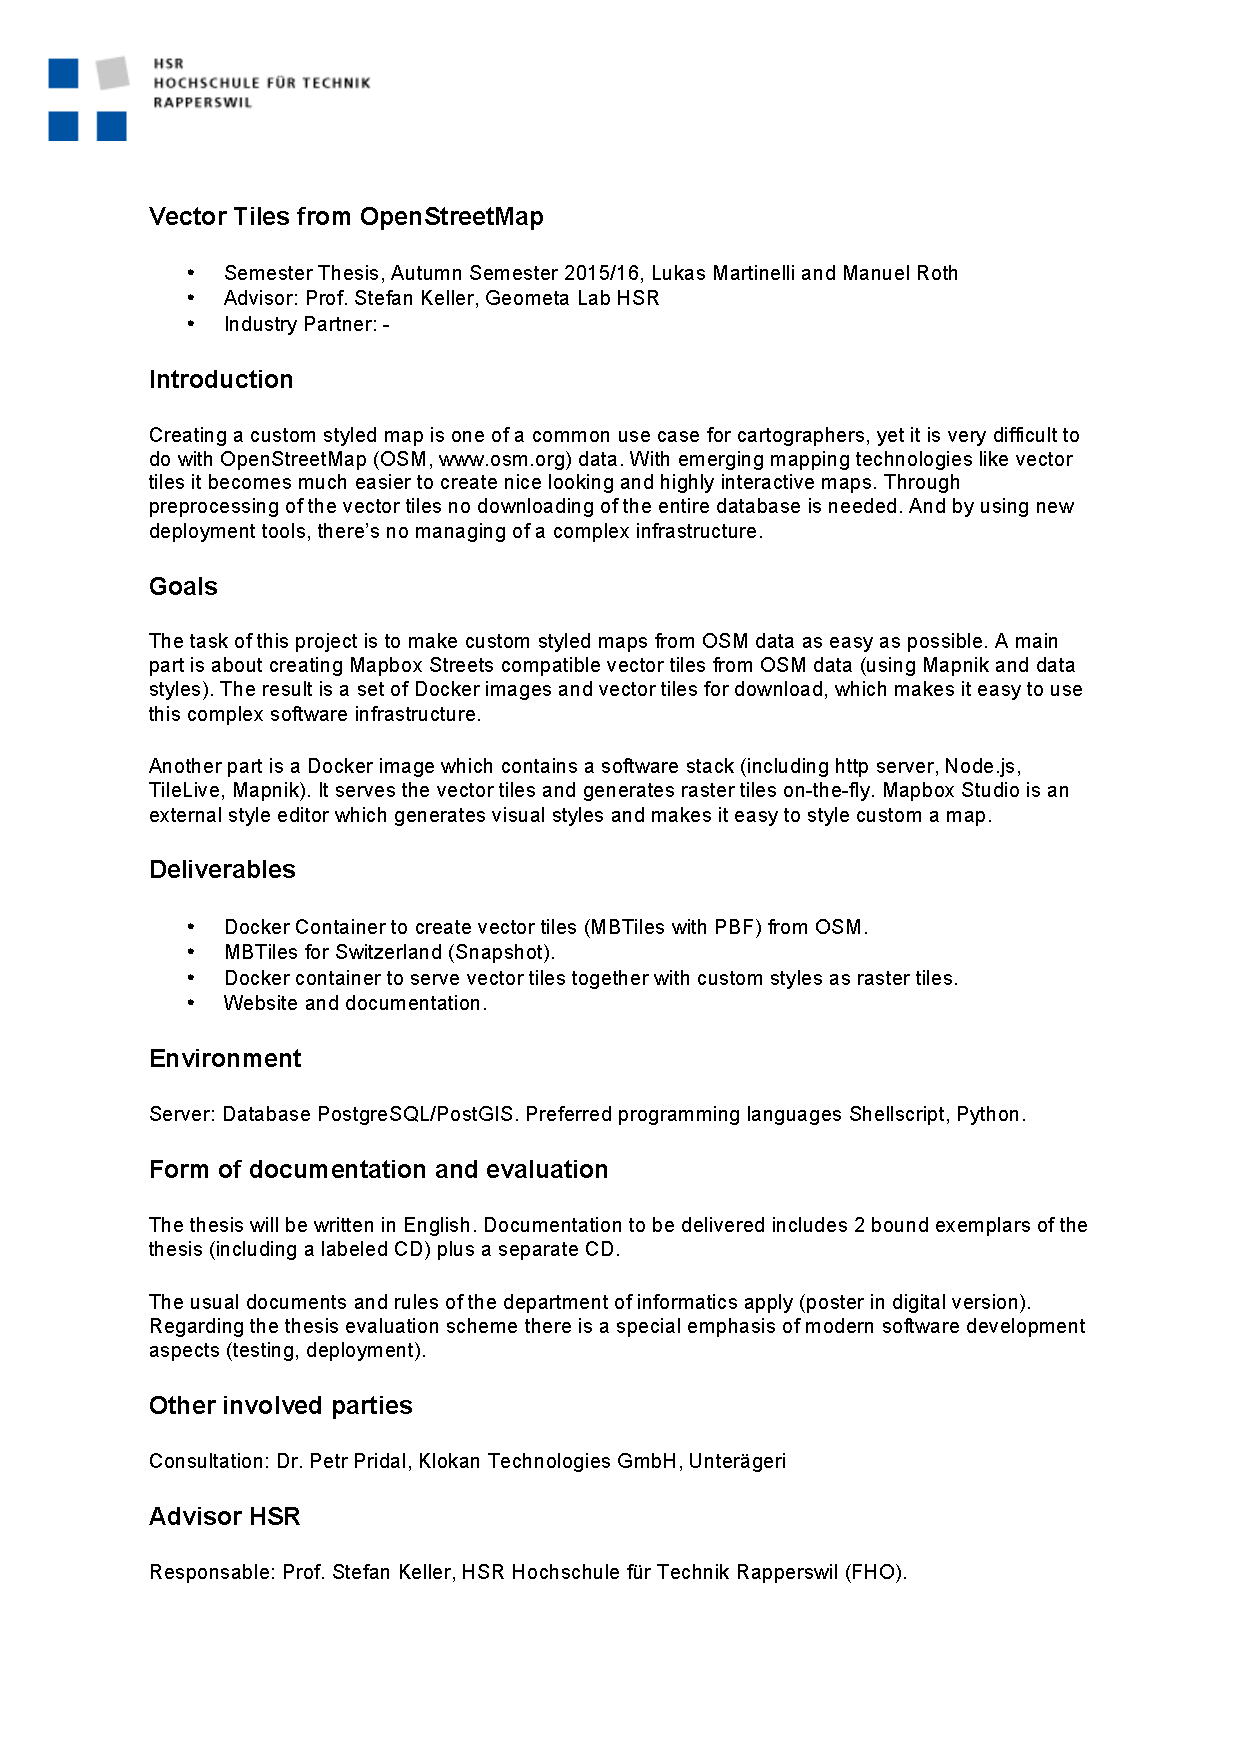
\includepdf[pages={1}]{images/project_proposal.pdf}

\pagestyle{scrheadings} % Show chapter titles as headings

% Table of Contents - List of Tables/Figures/Listings and Acronyms

\refstepcounter{dummy}

\pdfbookmark[1]{\contentsname}{tableofcontents} % Bookmark name visible in a PDF viewer

\setcounter{tocdepth}{2} % Depth of sections to include in the table of contents - currently up to subsections

\setcounter{secnumdepth}{3} % Depth of sections to number in the text itself - currently up to subsubsections

\manualmark
\markboth{\spacedlowsmallcaps{\contentsname}}{\spacedlowsmallcaps{\contentsname}}
\tableofcontents 
\automark[section]{chapter}
\renewcommand{\chaptermark}[1]{\markboth{\spacedlowsmallcaps{#1}}{\spacedlowsmallcaps{#1}}}
\renewcommand{\sectionmark}[1]{\markright{\thesection\enspace\spacedlowsmallcaps{#1}}}

\clearpage

\begingroup 
\let\clearpage\relax
\let\cleardoublepage\relax
\let\cleardoublepage\relax

%----------------------------------------------------------------------------------------
%	List of Figures
%----------------------------------------------------------------------------------------

\refstepcounter{dummy}

%\pdfbookmark[1]{\listfigurename}{lof} % Bookmark name visible in a PDF viewer

\listoffigures

\vspace*{8ex}
\newpage

%----------------------------------------------------------------------------------------
%	List of Tables
%----------------------------------------------------------------------------------------

\refstepcounter{dummy}
\listoftables

\vspace*{8ex}
\newpage
    
%-------------------------------------
%	List of Listings
%-------------------------------------

%\refstepcounter{dummy}

%\addcontentsline{toc}{chapter}{\lstlistlistingname} % Uncomment if you would like the list of listings to appear in the table of contents

%\pdfbookmark[1]{\lstlistlistingname}{lol} % Bookmark name visible in a PDF viewer
%
%\lstlistoflistings 
%
%\vspace*{8ex}
%\newpage
       
%----------------------------------------------------------------------------------------
%	Acronyms
%----------------------------------------------------------------------------------------
\refstepcounter{dummy}
\markboth{\spacedlowsmallcaps{Acronyms}}{\spacedlowsmallcaps{Acronyms}}
\chapter*{Acronyms}

\begin{acronym}[Acronyms]
\acro{OSM}{OpenStreetMap, free map}
\acro{ETL}{Extract, Transform and Load}
\acro{RUP}{Rational Unified Process}
\acro{GIS}{Geographic Information System}
\acro{GDAL}{Geospatial Data Abstraction Library}
\acro{WMS}{Web Map Service}
\acro{DRY}{Don't Repeat Yourself}
\acro{CI}{Continuous Integration}


\end{acronym}  

\newpage

%----------------------------------------------------------------------------------------
%	Glossary
%----------------------------------------------------------------------------------------
\refstepcounter{dummy}
\markboth{\spacedlowsmallcaps{Glossary}}{\spacedlowsmallcaps{Glossary}}
\chapter*{Glossary}

\begin{acronym}[Glossary]
\acro{Vector Tiles}{Packets of geographic data, packaged into pre-defined roughly-square shaped "tiles" for transfer over the web}
\acro{Data Style}{Description of feature classes such as landuse, water or roads}
\acro{Visual Style}{Definition of style rules for a specific schema, which is defined in the data style}
\acro{Feature Class}{Group of features with the same geometry type and attributes}
\acro{Layer}{Mapbox definition of a feature class}
\acro{Mapbox Streets}{Name of Mapbox's vector tile source}
\acro{MBTiles}{File format for storing map tiles in a single file}
\acro{GeoJSON}{File format for encoding a variety of geographic data structures}
\acro{Mapnik XML}{Stylesheet for the mapnik rendering engine}
\acro{CartoCSS}{Mapbox propritary cartographic styling language}
\acro{Mapbox GL}{Clientside rendering engine}
\acro{Web GL}{Javascript API for the graphics library in browsers}
\acro{Mapbox Studio Classic}{Client application to design custom maps}
\acro{OSM Bright}{Mapbox visual style}
\acro{Docker}{Operation system level virtualization on Linux}
\acro{Kitematic}{Client application for controlling docker containers}
\acro{Natural Earth}{Public map dataset}
\acro{OSM Planet}{All OpenStreetMap data in one file}






\end{acronym}  

\endgroup % Contents, list of figures/tables/listings and acronyms

\pagenumbering{arabic} % Arabic page numbering for thesis content (1, 2, 3, etc)

%------------------------------------------------
%	THESIS CONTENT - CHAPTERS
%------------------------------------------------
\newpage
\part{Technical Report} % First part of the thesis
\chapter{Introduction}

%-------------------------------------------------------

Creating a custom styled OSM map is one of the most common use cases
among cartographers yet it is very difficult to do so. With the new
emerging technology of vector tiles it is possible to allow anyone to
create their custom OSM maps without setting up a database and
managing complex infrastructure.

%------------------------------------------------------

\section{Vision}\label{part1_vision}

Michal Migurski published on March 15, 2013 a blog
post\cite{1_mike.teczno.com_2013},
in which he described his first attempts to use vector tiles as a source
for the Mapnik tile renderer and his vision for vector tiles.
\newline{}
Vector tiles only contain geometries and metadata.
The visual style is applied on the fly when the tile is requested, it is separated from the
actual vector data. Vector tiles are smaller than raster tiles, this enables high resolution maps, fast map loads and efficient caching.\cite{2_mapbox.com_2015} \\
Our mission is to bring the power of vector tiles to anyone and provide
the data free and as Open Source project.

%------------------------------------------------------

\section{Goals}\label{goals}

The main goal of this thesis is to allow anyone to create their custom
OSM map without managing complex infrastructure. In order to complete this goal
several deliverables were defined in the project proposal.

\begin{itemize}
\item
  Create workflow to create vector tiles from \osm{} data
\item
  Provide vector tiles for Switzerland
\item
  Provide method to serve the vector tiles together with
  custom styles as raster tiles
\item
  Optional: Vector tiles for the entire world
\end{itemize}

\paragraph{Differentiation} The resulting vector tiles allow creating an alternative base map, which is customizable. The vector tiles are not meant to be queried and do not support custom overlays. Additional map features need to be implemented with the help of other libraries. 
\chapter{State of Technology}

As of today most web maps are based on raster tiles except a few big providers like Google, Mapbox and Apple.
%\marginpar{The \hyperref[history-of-webmaps]{\emph{History of Webmaps}} chapter provides more details.}
The rest of the industry is now in the transition from raster based maps into vector based maps. For vector based maps the Mapbox Vector Tile Specification\footnote{\url{https://github.com/mapbox/vector-tile-spec/tree/master/1.0.1}} is the most dominant Open Source specification of vector tiles.

\section{Current Vector Data Providers}

While the deployment setup for vector based maps is much simpler than
the traditional raster tile setup the most complex part is still
the creation of vector data which takes a lot of time and care.

\paragraph{Mapbox}

Mapbox provides vector tiles of the entire world as part of its
map hosting technologies since 2012 branded as Mapbox Streets\footnote{\url{https://www.mapbox.com/blog/announcing-mapbox-streets/}}. Mapbox also provides the vector data for buyers of their Mapbox Atlas Server\footnote{\url{https://www.mapbox.com/atlas/}} starting at \$49,000 and distributes quarterly updates for \$10,000 per year .

\paragraph{Mapzen}

Mapzen provides API access to their public vector tiles\footnote{\url{https://mapzen.com/projects/vector-tiles/}}.
%\marginpar{Mapzen vector tiles can also be requested in GeoJSON, TopoJSON and Open Science Map format.}
Mapzen states that access and the platform should remain free and Open Source\footnote{\url{https://mapzen.com/about/}}. Mapzen however
does not give access to the entire raw data and one is bound to
the limitations of the service.

\paragraph{Kartotherian}

The Kartotherian\footnote{\url{https://www.mediawiki.org/wiki/Maps}} project from the Wikimedia Foundation\footnote{\url{https://wikimediafoundation.org/wiki/}} is very similar to this project.
The goal is to provide a free Map service that everyone can use for free.
The process is documented but the data is still bound to the service and not available as download.
The quality of the vector tiles is continuously improved but still lacking very important features.
Kartotherian is a great project which we can contribute to with our improved map data.

\paragraph{Google and Apple}

Apple started using vector tiles in their Apple Maps product in 2012\cite{wiki:apple-maps}  and  Google is using vector tiles since 2013\cite{wiki:google-maps} but they are both not accessible for the general public and use a proprietary format. 

\section{Characteristics}

While the providers open the process they still own the data in order to keep their strategic advantages and promote the use of their products using this data.
The open process is a wonderful step in the right direction, yet it requires great understanding
of the technology and sufficient computing power to actually
execute the workflow of producing vector tiles with worldwide coverage.

\section{Shortcomings}

The providers already solve the problem of producing the vector tiles
and making it accessible. The data however can only be used
via their services.
\newline{}
Being able to download world data and use it in a custom server
infrastructure, offline and without strings attached is a big advantage
and a problem this thesis wants to solve.

\newpage
\chapter{Implementation Concept}\label{implementation_concept}

The implementation is divided into the vector tile rendering process and the tile server. The following two sections describe the high level concept of both implementations.

\section{Vector Tile Rendering}

\paragraph{Import}
In the import phase data sources are imported into a spatial database and mapped to a database schema.

\paragraph{Export}
In the export phase a data style is applied to the database to produce vector tiles.

\paragraph{Data Style}
\marginpar{The section \hyperref[data_style]{\emph{Data Style}} in part two provides more details.}The data style is a description of the vector tile structure and the SQL queries to fetch the data.

\begin{figure}[h]
  \centering
  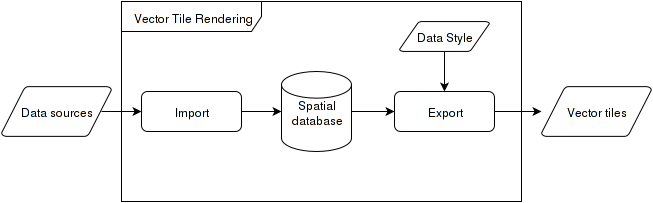
\includegraphics[scale=0.6]{images/vector_tile_rendering_squashed.png}
  \caption{Vector Tile Rendering Process}
\end{figure}

\section{Tile Server}

To display the vector tiles a tile server and a visual style is needed. There are two possibilities, which are described in the following two sections.

\paragraph{Visual Style}
The visual style defines how a feature class such as landuse actually gets displayed. In the case of landuse on could define the texture or the color of the border and area.


\subsection{Raster Tile Server}

The raster tile server makes it possible to display the vector tiles. It takes the visual style (CartoCSS\footnote{\url{https://github.com/mapbox/carto/blob/master/docs/latest.md}}) and the vector tiles as input. The renderer generates raster tiles of these inputs. When a raster tile is rendered, it is served by the webserver. Any GIS Software which supports raster tiles can consume the raster tiles served by the server.

\begin{figure}[h]

  \centering
  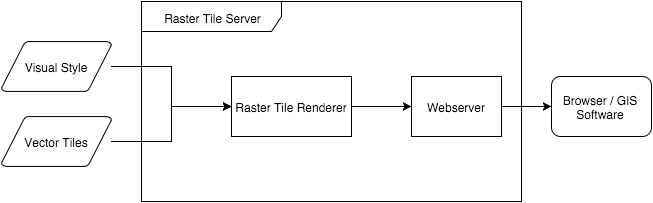
\includegraphics[width=1\textwidth]{images/raster_tile_server.png}
  \caption{Raster tile server}
\end{figure}

\subsection{Vector Tile Server}

The vector tile server in contrast to the raster tile variant directly serves the vector tiles to the client. The raster tiles are rendered on the client side using visual style. The advantage of this approach is more control over the user experience and that less server computing power is needed.

\begin{figure}[h]

  \centering
  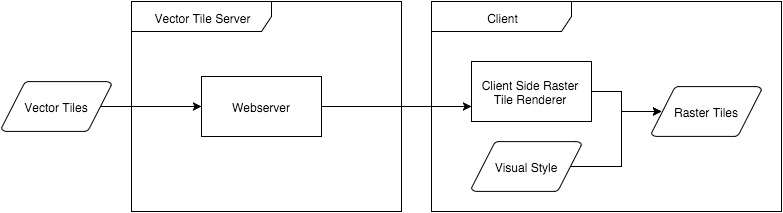
\includegraphics[width=1\textwidth]{images/vector_tile_server.png}
  \caption{Vector tile server}
\end{figure}

\newpage
\chapter{Results and Future}\label{part1_results_and_future}

All objectives which we defined in \hyperref[goals]{\nameref{section 1.2}} have been achieved. The optional goal to provide vector tiles for the entire world has been moved to the bachelor thesis.

\section{Results}\label{part1_results}

\begin{itemize}
\item
  Docker containers and documentation for the entire workflow of creating vector tiles has been created.
\item
  The raster tile server for serving the vector tiles together with a visual style has been realized.
\item
  The project website with information about how to use the vector tiles is online.
\end{itemize}

The vector tiles for Switzerland can be downloaded from the project website (\url{http://osm2vectortiles.org}). These vector tiles can be served together with a visual style in our vector tile server.
\newline{}
A custom visual style can be created with Mapbox Studio Classic\cite{mapbox_studio_classic}.
All existing visual styles based of Mapbox Streets are compatible with the produced vector tiles. This allows very easy migration to osm2vectortiles.

\begin{figure}[H]
  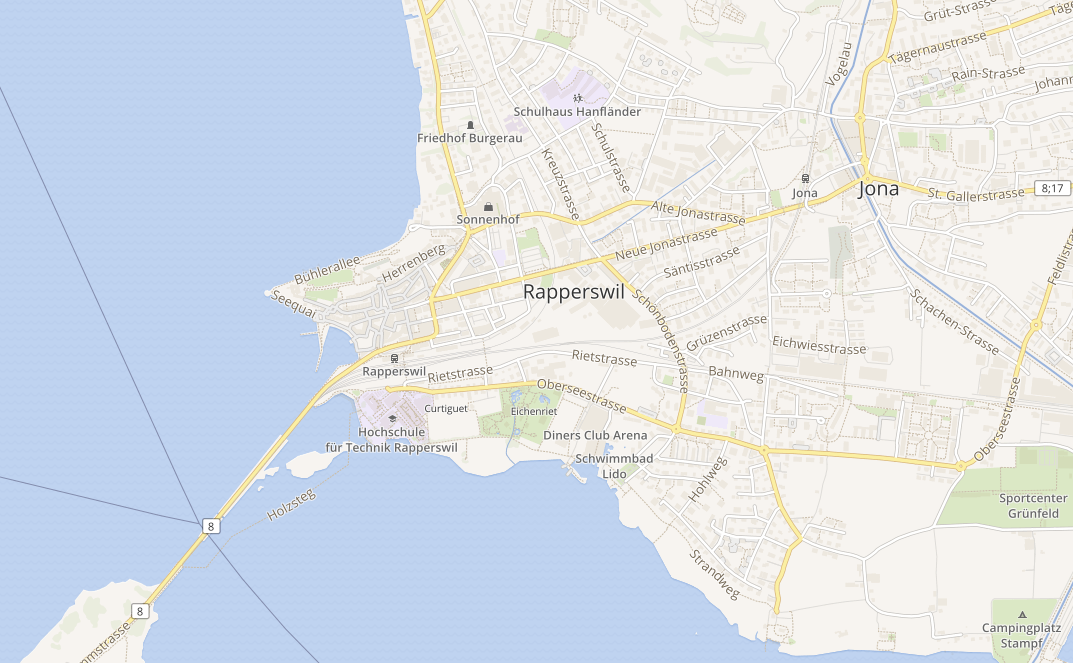
\includegraphics[width=1\textwidth]{images/unmodified_osm_bright.png}
  \caption{Unmodified OSM Bright visual style using osm2vectortiles}
\end{figure}

\section{Future}\label{part1_future}
In a first step the project should be expanded to provide vector tiles for the entire world. The vector tile rendering workflow needs to be scaled out for the entire world. Regular updates for the vector tiles have been requested by the members of the Swiss OSM community
and will require identifying and rerendering updated tiles.\\
The long-term vision of this project is to provide a complete offline map experience, including basic geographic name search. These suggestions will be the project goals for the bachelor thesis. More detailed listing of
future features can be found in \autoref{part2_results_and_future}.


%------------------------------------------------
\newpage
\part{Project Documentation}
\chapter{Vision}\label{vision}

The vision of our project is described in part 1, section~\ref{vision}. This chapter should give a bit of background on where the idea of vector tiles came from.

\section{History of Webmaps}
\label{history-of-webmaps}

Web mapping has gone through different technological changes in recent years. It is important to understand the evolution of web maps to understand why vector tiles are quite a fundamental change in how maps work.

\paragraph{Phase 1: Untiled Static
Maps}

In the beginning WMS servers generated static images for an extract
of the map. Each view of a map requested a unique extract of a map that was generated for this person.

\paragraph{Phase 2: Raster Tiles}

In 2005 Google introduced Google Maps and XYZ 
tiles\footnote{\url{http://wiki.openstreetmap.org/wiki/Slippy_Map}}
which delivered a idempotent raster image for coordinates specified by a
tile index.

\paragraph{Phase 2.5: Raster Tiles with Vector
Overlays}

To provide a level of interactivity, tools like
Leaflet\footnote{\url{http://leafletjs.com/}} support rendering vector
data like SVG on top of a raster based maps.

\paragraph{Phase 2.75: Raster Tiles from Vector
Tiles}

For backwards compatibility and faster serving of raster tiles vector
tiles where introduced to avoid querying a database.

\paragraph{Phase 3: Vector Tiles}

Vector tiles are delivered directly to the browser and rendered by Web
GL based clients.
\newline{}
Improving the use of vector data in web mapping is often shown as the next challenge
of web mapping \cite[p.~88]{gaffuri2012toward} 
\newpage
\chapter{Requirements Specification}\label{requirements_specification}

This chapter describes the requirements for the vector tiles and the vector tile server.

\section{User Characteristics}\label{user_characteristics}

There are three user groups interested in this project:

\begin{itemize}
\item
  \textbf{Map Designer}: A technically versed person using Windows or
  OSX with knowledge of GIS software but not necessarily of it's
  inner technical workings.
\item
  \textbf{System Administrator}: The person which needs to host the
  published maps.
\item
  \textbf{Geographic Institutes or other companies}: Institutions which would like to provide their own geospatial data in vector tile format. 
\end{itemize}

\section{User Stories}\label{user_stories}
\paragraph{Serverside Rendering}
The map designer brings his new map design to the system administrator and tells him to host the map. The system administrator can download the vector tiles of the osm2vectortiles website and serve the map with the help of a vector tile server.

\paragraph{Clientside Rendering}
The map designer brings his new map design to the system administrator and tells him to host the map. The system administrator does not want to provide a big server that can handle the heavy rendering work. So he decides to use Mapbox GL\footnote{\url{https://www.mapbox.com/mapbox-gl-js/api/}} which offloads the rendering work to the client. In order to use Mapbox GL he needs to statically serve the vector tiles. 

\paragraph{Own vector tiles}
Institutions which provide geospatial data would like to follow the trend of vector tiles and provide their data in vector tile format. These institutions can use this project for this matter. They can easily modify this project to use it with their data. 

\section{Non Functional Requirements}\label{non_functional_requirements}

The non functional requirements are the key to success of this project. If we can fulfill the following requirements, the specified users will be able to benefit form our project.

\paragraph{Usability}
The vector tile server must be usable with Kitematic\footnote{\url{https://kitematic.com/}}. Kitematic is an easy to use user interface for docker. 

\paragraph{Learnability}

Map designers should not have to learn how to use the command line in
order to use Docker.

\paragraph{Repeatable}

Generating OSM vector tiles must be possible in a weekly interval because OSM
updates regularly.

\paragraph{Performance}

The tileserver must handle 10 concurrent users per second.

\paragraph{Compatibility}

The vector tiles must contain all feature sets Mapbox Streets contains. If we can guarantee full compatibility with Mapbox Streets\footnote{\url{https://www.mapbox.com/developers/vector-tiles/mapbox-streets-v6/}} all Mapbox visual styles can be used with our vector tiles.

\paragraph{Vector Tile Size}

The size of a single vector tile should not be greater than 500 KB.
\newpage
\chapter{Design}\label{design}


%------------------------------------------------------
\section{Architecture}\label{architecture}



%------------------------------------------------------
\section{Database Schema}\label{database-schema}


The schema is flat and has no relations. Each table contains
information about its entity and geometry. Because imposm 3
cannot match two types of polygons (e.g. polygon and point) we need
to create a table for each geometry type.


\subsection{Common Attributes}

\subsubsection{OSM id}

All tables and views that are derived from \osm{} data have keep the original \texttt{osm\_id}
to trace back the data and be able to query a distinct \osm{} feature in a visual style.

\subsubsection{Translations}

All features that will get a label layer will contain several translations.

\begin{flushleft}
\begin{table}
    \begin{tabular}{ll}
    \hline
     Field    & 	Description                                    \\
    \hline
    name      & Local name for the place.  \\
    name\_en	 & English                          \\
    name\_es	 & Spanish                          \\
    name\_fr	 & French                           \\
    name\_de	 & German                           \\
    name\_ru	 & Russian                          \\
    name\_zh	 & Chinese                          \\
    \end{tabular}
\end{table}
\end{flushleft}


\subsubsection{Type and Class}

The class can be explained as a feature class. It is a categorization of a OSM value.
The type is the OSM value of the feature.


\subsection{OpenStreetMap Planet}

\begin{flushleft}
    \begin{tabular}{lll}
    \hline
    Table Name            & Geometry Type & Description \\
    \hline                                          
    admin                  & linestring    & Administrative boundaries \\
    buildings              & polygon       & Building shapes                            \\
    landusages             & polygon       & Human use of land \\
    places                 & point         & Populated settlements                      \\
    roads                  & linestring    & Roads, tracks and paths          \\
    aero\_lines            & linestring    & Airports and aviation-related items        \\
    aero\_polygons         & polygon       & see aero\_lines                            \\
    barrier\_lines         & linestring    & Movement blocking structures   \\
    barrier\_polygons      & polygon       & see barrier\_lines                         \\
    housenumbers\_points   & point         & Address information about houses \\
    housenumbers\_polygons & polygon       & see housenumbers\_points                   \\
    poi\_points            & point         & Point of interest                          \\
    poi\_polygons          & polygon       & see poi\_points                            \\
    water\_lines           & linestring    & Lakes and rivers                           \\
    water\_polygons        & polygon       & see water\_lines                           \\
    \end{tabular}
\end{flushleft}

\subsection{Custom Curated Data}

Certain data is very delicate and has been added by hand.

\begin{flushleft}
    \begin{tabular}{lll}
    \hline
    Table Name   & Geometry Type & Description \\
    \hline                                          
    marine       & point    & Marine names \\
    countries    & point    & Country names \\
    states       & point    & State names \\
    \end{tabular}
\end{flushleft}

\subsection{OpenStreetMapData}

We use the the water polygons\footnote{\url{http://openstreetmapdata.com/data/water-polygons}} 
from OpenStreetMapData for oceans, seas and large lakes.

\begin{flushleft}
    \begin{tabular}{lll}
    \hline
    Table Name            & Geometry Type & Description \\
    \hline
    water\_polygons        & polygon       & Ocean, seas, large lakes           \\
    \end{tabular}
\end{flushleft}


\subsection{Natural Earth}


The imported natural earth data results in more than 100 tables but only a few
are relevant for our use case.
We use country, state borders and large lakes from Natural Earth data for the lower zoom
levels.


\begin{flushleft}
    \begin{tabular}{ll}
    \hline
    Table Name                                          & Geometry Type \\
    \hline
    ne\_110m\_admin\_0\_boundary\_lines\_land           & linestring    \\
    ne\_50m\_admin\_0\_boundary\_lines\_land            & linestring    \\
    ne\_10m\_admin\_0\_boundary\_lines\_land            & linestring    \\
    ne\_50m\_admin\_1\_states\_provinces\_lines         & linestring    \\
    ne\_10m\_admin\_1\_states\_provinces\_lines\_shp    & linestring    \\
    ne\_10m\_admin\_0\_boundary\_lines\_disputed\_areas & linestring    \\
    ne\_110m\_lakes                                     & polygon       \\
    ne\_50m\_lakes                                      & polygon       \\
    ne\_10m\_lakes                                      & polygon       \\
    \end{tabular}
\end{flushleft}

%------------------------------------------------------
\newpage
\section{Layer Schema}\label{layer-schema}

\begin{flushleft}
    \begin{tabular}{ll}
    \hline
     Layer             & Description                     \\
    \hline
    \#landuse          & Both land-use and land-cover.   \\
    \#waterway         & Rivers                          \\
    \#water            & Oceans and seas                 \\
    \#aeroway          & Aero related lines and polygons \\
    \#barrier\_line    & Barrier lines and polygons      \\
    \#building         & Building polygons               \\
    \#landuse\_overlay & Transparent overlays for water  \\
    \#tunnel           & Tunnels                         \\
    \#road             & Roads                           \\
    \#bridge           & Bridges                         \\
    \#admin            & Administrative borders          \\
    \#country\_label   & Labels of countries             \\
    \#marine\_label    & Labels of oceans and seas       \\
    \#place\_label     & Labels of places                \\
    \#water\_label     & Labels of lakes                 \\
    \#poi\_label       & Labels of point of interest     \\
    \#road\_label      & Labels of roads                 \\
    \#waterway\_label  & Labels of rivers                \\
    \#housenum\_label  & Labels of housenumbers          \\
    \end{tabular}
\end{flushleft}

\newpage
\subsection{Aeroways, Barriers and Landusages}

For alot of layers linestring and polygon data needs to be converted into
linestrings for the layers.

\begin{figure}[h]
  \centering
  \includegraphics[scale=0.6]{images/aero_barrier_landusage_layer.png}
  \caption{Layers for aeroways, barriers and landusages}
\end{figure}

\newpage
\subsection{Administrative Borders}
Administrative area at lower zoom levels is entirely from Natural Earth.

\begin{figure}[h]
  \centering
  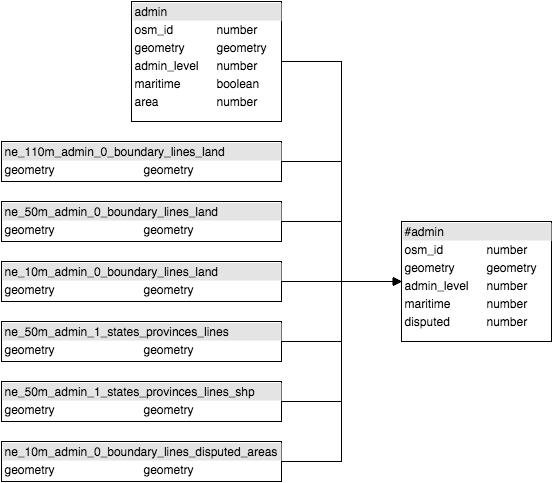
\includegraphics[scale=0.6]{images/admin_layer.png}
  \caption{Layers for administrative areas}
\end{figure}

\newpage
\subsection{Roads, Bridges and Tunnels}
Roads are split up into normal roads, tunnels and bridges after a certain zoom level. \texttt{z\_order} and \texttt{layer} attributes are used to order the geometries on the right z axis.

\begin{figure}[h]
  \centering
  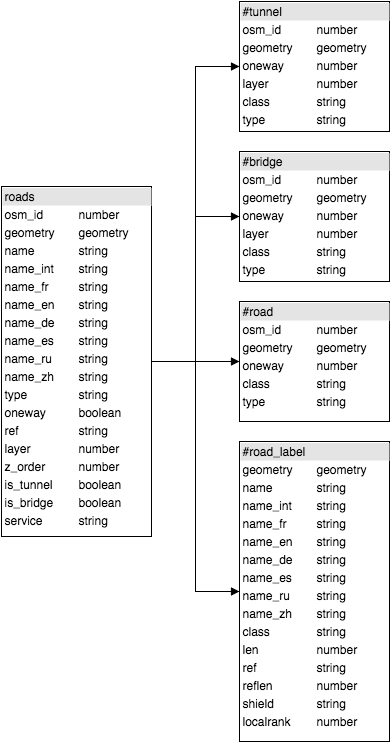
\includegraphics[scale=0.6]{images/road_layer.png}
  \caption{Layers for roads, tunnels and bridges}
\end{figure}

\newpage
\subsection{Points of Interest}
Most POIs are in fact points but buildings tagged with POI attributes
are often polygons, which is why we need to create tables for both points and polygons.
The \texttt{localrank} and \texttt{scalerank} of the \texttt{\#poi\_label} layer are calculated from the \texttt{type} and \texttt{area} attributes.
The \texttt{address} field is pulled together from the various address attributes on the tables (\texttt{street}, \texttt{housenumber}, \texttt{place}, \texttt{city}, \texttt{postcode} and \texttt{country}).

\begin{figure}[h]
  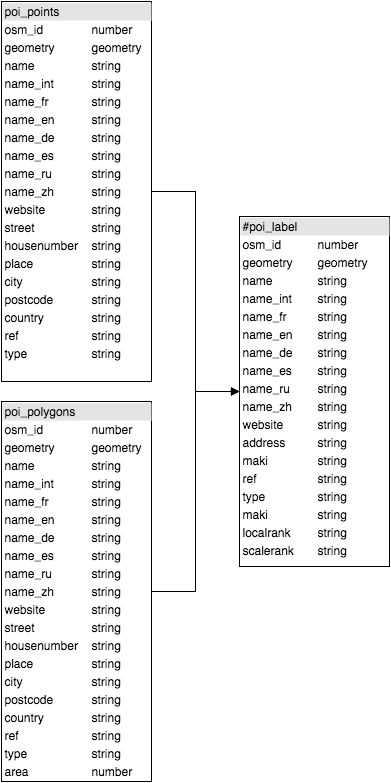
\includegraphics[scale=0.6]{images/poi_layer.png}
  \caption{Point of interest label layer}
\end{figure}


\newpage
\subsection{Water}
Water bodies for lower zoom levels are taken from Natural Earth
data while lakes and rivers are from \osm{}.

\begin{figure}[h]
  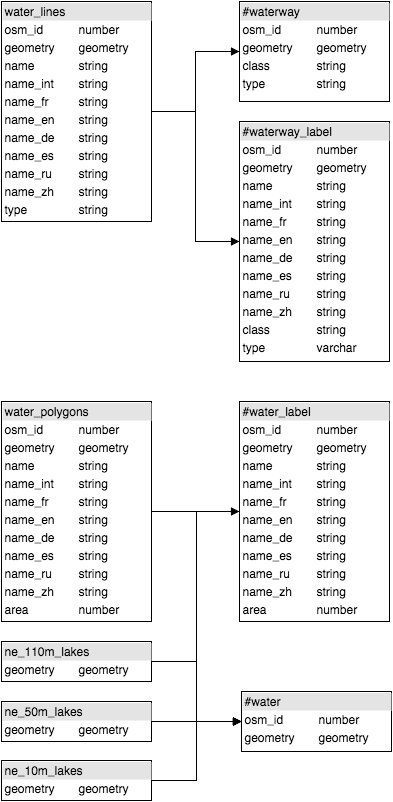
\includegraphics[scale=0.6]{images/water_layer.png}
  \caption{Water bodies and river layers}
\end{figure}



\newpage
\subsection{Places}
The original \osm{} place data is enriched with scalerank data
from natural earth.

\begin{figure}[h]
  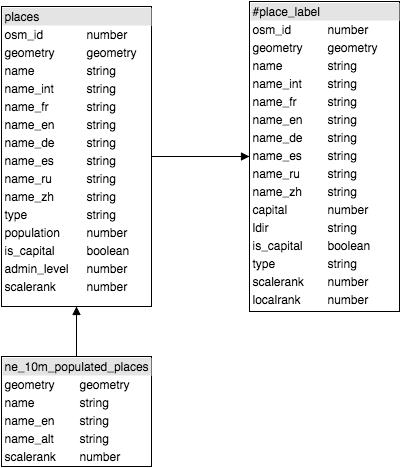
\includegraphics[scale=0.6]{images/place_layer.png}
  \caption{Place label layer}
\end{figure}



%------------------------------------------------------
\newpage
\section{Package Diagrams}

\subsection{Import}

The entire import process is a combination of different smaller imports of different datasources.

\paragraph{import-osm-data}
Import of the OSM planet file with imposm 3 and a custom mapping configuration.

\paragraph{import-sql}
Custom SQL functions that make querying easier and generated SQL code for
classifications.

\paragraph{import-natural-earth}
Import of Natural Earth data.

\paragraph{import-scaleranks}
Custom scalerank updates from Natural Earth data for better scaleranks in places.

\paragraph{import-water}
Water polygons from OpenStreetMapData.

\begin{figure}[h]
  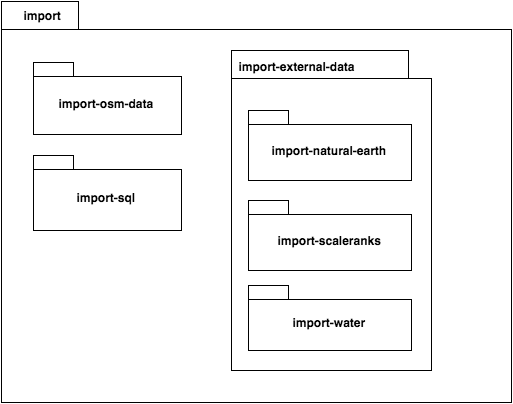
\includegraphics[scale=0.6]{images/import_package.png}
  \caption{Import package}
\end{figure}

\newpage
\subsection{Export}
Export can either be done locally which will process one bounding box or
split up into several machines using remote features.

\paragraph{open-streets.tm2source}
The data style project is the most essential component which pulls together all the
data of different datasources to create vector tile. 

\paragraph{export-local}
A process which is using the open-streets.tm2source project to create vector tiles for a
given bounding box.

\paragraph{export-remote}
A worker implementation which uses a queue to read jobs and work through jobs with
export-local.

\paragraph{enqueue-jobs}
Create jobs for certain areas automatically.

\paragraph{merge}
Merge results of jobs together into a final big file.

\begin{figure}[h]
  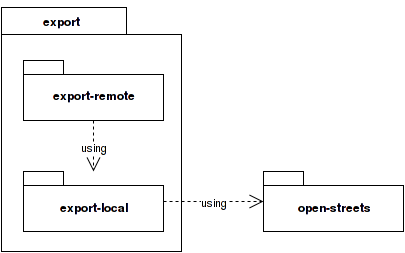
\includegraphics[scale=0.6]{images/export_package.png}
  \caption{Export package}
\end{figure}

%------------------------------------------------------
\section{Workflow}\label{workflow}

\paragraph{First step: Getting OSM
data}\label{first-step-getting-osm-data}

There are many different sources available to get \osm{} data from. Most of
the time Geofabrik\footnote{\url{http://download.geofabrik.de/}} was
referenced for getting single countries, continents or even the whole
planet. But many times people only need a single city or region, because
of this demand
Mapzen\footnote{\url{https://mapzen.com/data/metro-extracts/}} provides
OSM data for many cities and regions around the globe.

The \osm{} data is missing something very important: the administrative
boundaries. This needs to be downloaded separatly due to the fact, that
somebody could manipulate the boundary of a region. As a result of this
administrative boundaries get checked by the \osm{} community and released
separatly.

The data is available in the PBF and \osm{} XML format. If available the
PBF(Protocolbuffer Binary
Format)\footnote{\url{http://wiki.openstreetmap.org/wiki/PBF_Format}}
version should be choosen, as it is 30\% smaller and 5-6 times faster to
read and write than the bzipped \osm{} XML version.

\paragraph{Second step: Importing \osm{} data into
Postgis}\label{second-step-importing-osm-data-into-postgis}


\subsubsection{Third step: Mapbox studio source
project}\label{third-step-mapbox-studio-source-project}

A Mapbox studio source project is divided into the following folder
structure\footnote{\url{https://www.mapbox.com/guides/source-manual/\#source-project}}:

\begin{verbatim}
source-project.tm2source/
    data.yml
    data.xml
    .thumb.png
\end{verbatim}

The data file defines all feature sets(layers) like landuse, waterway,
road etc. The definition contains metadata like id, datasource(db, host,
query, srid, extent), description, fields and properties. Mapbox Studio
needs the yml version and mapnik the xml version of this file.
.thumb.png is a thumbnail image that gets displayed in the projects
list.

\subsubsection{Fourth step: Generating vector
tiles}\label{fourth-step-generating-vector-tiles}

To generate the vector tiles we use mapnik. Mapbox provides a very handy
tool to generate vector tiles.

\begin{verbatim}
tilelive-copy --bounds=-180,-85,180,85 bridge:///home/mapbox/tmp/project.tm2source/data.xml mbtiles:///tmp/project.mbtiles
\end{verbatim}

tilelive-copy provides the Mapnik XML file and the extent to mapnik
which then generates the vector tiles. Tilelive-copy outputs these
vector tiles in the mbtiles container.
\newpage
\chapter{Technology Evaluation}\label{technology_evaluation}

\section{Spatial Database}\label{spatial_database}

The OSM wiki\footnote{\url{http://wiki.openstreetmap.org/wiki/Databases_and_data_access_APIs\#Database_Schemas}} recommends PostgreSQL with the PostGIS extension for processing the data. There also exists a method\footnote{\url{https://github.com/systemed/tilemaker}} that circumvents using a database and directly transform OSM data into vector tiles but this does not scale for global vector tile coverage and does not support mixing additional data into the vector tiles.

\\
\begin{tcolorbox}[arc=0mm,boxrule=1pt,title=Decision]\label{spatial_db_decision}
PostGIS was the only viable choice due to superb tooling support for OSM data and
advanced spatial query capabilities.
\end{tcolorbox}

\section{OSM Import Tool}\label{osm_import_tool}
As import tool the OSM community recommends imposm\footnote{\url{http://imposm.org/}} or osm2pgsql\footnote{\url{http://wiki.openstreetmap.org/wiki/Osm2pgsql}}.
In this section the two tools are compared with each other.

\subsection{Criterias}\label{criterias}

\paragraph{Speed} 
In order to iterate fast and be able to change the data style frequently
it is important that the import tool is reasonably fast and is able
to import the OSM planet file in one single day.

\paragraph{Customized Schema}
Customizing a schema to already split up features into separate tables
makes querying more performant and easier to do.

\paragraph{Diff Updates}
It must be possible to apply the Planet diffs \footnote{\url{http://wiki.openstreetmap.org/wiki/Planet.osm/diffs}} 
to continuously update the database with newer data.
\\
If a import is very fast it is also possible to simply reimport the latest
planet dump.

\paragraph{Existing Data Style Projects}
In order to get started it is helpful to have a lot of query examples
from other data style projects available.

\subsection{Evaluation Matrix}\label{evaluation_matrix}

\begin{table}[H]
\centering
    \begin{tabular}{llll}
    \hline
    Criteria         & Weight & imposm & osm2pgsql \\
    \hline
    Speed             & 0,3    & 8      & 5         \\
    Customized Schema & 0,4    & 7      & 4         \\
    Diff Updates      & 0,2    & 6      & 8         \\
    Existing Material & 0,1    & 6      & 10        \\
    \hline
    \textbf{Weighted Score} & 1      & 7      & 5,7       \\
    \end{tabular}
    \caption{Evaluation matrix of imposm vs osm2pgsql}
\end{table}


\subsection{osm2pgsql}\label{osm2pgsql_importer}

osm2pgsql\footnote{\url{http://wiki.openstreetmap.org/wiki/Osm2pgsql}} is the
most commonly used import tool for processing raw OpenStreetMap data into PostGIS.
The import schema is also called osm2pgsql and defines a very
simple schema(line, point, polygon and
roads)\footnote{\url{http://wiki.openstreetmap.org/wiki/Osm2pgsql/schema}}.
This results in very large tables, so it is recommended to create good
indices. Osm2pgsql supports updating of the database, if the values have
been stored as hstore. The schema can be adapted via the import style \footnote{\url{http://wiki.openstreetmap.org/wiki/Osm2pgsql\#Import_style}}
but most projects use the default style\footnote{\url{https://github.com/openstreetmap/osm2pgsql/blob/master/default.style}} provided by osm2pgsql.

\subsubsection{imposm3}\label{imposm-importer}

Imposm is an import tool for OSM data, it is not a schema. But it
defines a default
schema\footnote{\url{http://imposm.org/docs/imposm/latest/database_schema.html}},
which could possibly be changed by provinding a custom mapping file. An
advantage of the default schema is that it groups data thematically into
tables. Which results in smaller tables and simpler queries. Imposm 3
supports updating the database from OSM diff
files\footnote{\url{http://imposm.org/docs/imposm3/latest/tutorial.html\#diff}}

\\ 
\begin{tcolorbox}[arc=0mm,boxrule=1pt,title=Decision]\label{osm_import_tool_decision}
For the use case of this thesis it is important, that the import is efficent and that
the import tool supports updating based on OSM diff files. Imposm3 is
faster than osm2pgsql and supports updatability and therefore it was decided to use imposm3 for importing.
\end{tcolorbox}

\section{Vector Tile Format}\label{vector-tile-formats}

Vector tiles are a broad term. In this thesis vector tiles correspond to Mapbox vector tiles which is a custom open specification how vector tiles should be structured.

\paragraph{Mapbox Vector Tiles}

When Mapbox introduced it's geography tool Mapbox Studio in 2013 they
created the \emph{Mapbox Vector Tiles Specification}
\footnote{\url{https://github.com/mapbox/vector-tile-spec}} which is
implemented by a variety of tools and clients
\footnote{\url{https://github.com/mapbox/awesome-vector-tiles}}
including \emph{Mapbox GL JS}, \emph{Open Layers 3}, \emph{Leaflet},
\emph{Mapzen Tangram} and Esri
\footnote{\url{https://www.mapbox.com/blog/vector-tile-adoption/}} in
the future.

\paragraph{Geopackage}

The \emph{GeoPackage Encoding Standard} is the OGC counterpart to the
\emph{Mapbox Vector Tiles Specification} which was introduced later and
is supported by QGIS, ESRI and GDAL.

\paragraph{Google Maps}

Google Maps is using vector tiles since 2010 under the hood and was the
first provider implementing this. Styling is limited and the format
proprietary.

\\
\begin{tcolorbox}[arc=0mm,boxrule=1pt,title=Decision]\label{vector_tile_spec_impl_decision}
Because one of the main requirements of this project was to provide Mapbox Streets compatible vector tiles and Mapbox provides very good tools to handle vector tiles, there was no other choice than going with Mapbox's implementation of vector tiles.
\end{tcolorbox}

\section{Vector Tile Server}\label{vector_tile_server}

Next to the vector tiles for Switzerland, the second deliverable is a basic vector tile server. The goal is that a non technical person can get started quickly with the custom vector tiles.\\

Unlike the choice for a spatial database or OSM import tool
there is no typical setup method of a raster tile server using vector tiles under the hood. Most people in the Open Source community build their own specific tile server setup.

\subsection{Tessera}\label{tessera}

Tessera\footnote{\url{https://github.com/mojodna/tessera}} is a Node.js\footnote{\url{https://nodejs.org/en/}} webserver, which s using Mapbox tilelive\footnote{\url{https://github.com/mapbox/tilelive}} modules to read vector tiles and generates raster tiles.

\begin{figure}[H]
\centering
  \includegraphics[scale=0.6]{images/tessera_node_bindings.png}
  \caption{Architecture Diagramm Tessera}
\end{figure}

Load tests were performed to measure server performance with tessera.
\\
\textbf{Infrastructure}: AWS EC2 t2.micro instance(1 GB Memory / 1 Core)
\textbf{Task}: Zooming in from zoom level 10 to 22 \\
\textbf{Conditions}: 50 concurrent users \\

A sample result of the load test is shown below.

\begin{bashcode}
---- Global Information --------------------------------------------------------
> request count                                      10350 (OK=10348  KO=2     )
> min response time                                     50 (OK=50     KO=60010 )
> max response time                                  60335 (OK=56103  KO=60335 )
> mean response time                                  2138 (OK=2127   KO=60172 )
> std deviation                                       3023 (OK=2914   KO=162   )
> response time 50th percentile                       1115 (OK=1114   KO=60172 )
> response time 75th percentile                       3127 (OK=3125   KO=60253 )
> mean requests/sec                                 75.919 (OK=75.904 KO=0.015 )
---- Response Time Distribution ------------------------------------------------
> t < 800 ms                                          4545 ( 44%)
> 800 ms < t < 1200 ms                                 756 (  7%)
> t > 1200 ms                                         5047 ( 49%)
> failed                                                 2 (  0%)
---- Errors --------------------------------------------------------------------
> java.util.concurrent.TimeoutException: Request timed out to ec      2 (100.0%)
2-52-30-184-45.eu-west-1.compute.amazonaws.com/52.30.184.45:80...
\end{bashcode}

With 50 concurrent users tessera was still able to respond to all requests in less than 1200 ms.

\subsection{OpenStreetMap "Standard" Tile Server}\label{osm_standard_tile_server}

A proven set up for generating raster tiles directly from PostgreSQL with Mapnik consists of an Apache webserver and a custom Apache module mod\_tile\footnote{\url{http://wiki.openstreetmap.org/wiki/Mod_tile}}. This approach was around before vector tiles were proposed.

\begin{figure}[H]
\centering
  \includegraphics[scale=0.6]{images/mod_tile.png}
  \caption{Architecture Diagramm OSM Standard tile server}
\end{figure}

It is theoretically possible to implement a raster tile server
on top of Mapnik and renderd using C++. Instead of using a spatial database as source for the rendered raster tiles a datasource binding would need to be implemented to read the vector tiles and hand them over to the Mapnik renderer. 

\\
\begin{tcolorbox}[arc=0mm,boxrule=1pt,title=Decision]\label{tile_server_decision}
The plan was to perform the load test on each version of the vector tile server and then make the decision based on the results. Due to the fact, that the test results of tessera where good enough for the thesis use case and it didn't take much time to implement, it was decided to use tessera as raster tile server.
If somebody needs a high-performance tile server, one should probably think about the second variant.
\end{tcolorbox}\newpage
\chapter{Implementation}\label{implementation}

The most promising vector tile specification was proposed by Mapbox.
\marginpar{The Mapbox Vector Tile Specification is compared with other vector tile formats in chapter \ref{vector-tile-formats}}
They provide many open source tools to manage vector tiles. We tried not to implement tools which already exists and instead use as many existing tools as possible. Because of this our implementation consists mostly of docker containers which do a specific task.

\section{Workflow}\label{workflow}
This section describes the workflow of generating vector tiles. The following sections will provide implementation details on each of the steps described here. 

\paragraph{First step: Getting OSM data}

There are many different sources available to get OSM data from. Most of
the time Geofabrik\footnote{\url{http://download.geofabrik.de/}} was
referenced for getting single countries, continents or even the whole
planet. But many times people only need a single city or region, because
of this demand
Mapzen\footnote{\url{https://mapzen.com/data/metro-extracts/}} provides
OSM data for many cities and regions around the globe.

The OSM data is missing something very important: the administrative
boundaries. This needs to be downloaded separatly due to the fact, that
somebody could manipulate the boundary of a region. As a result of this
administrative boundaries get checked by the OSM community and released
separatly.

The data is available in the PBF and OSM XML format. If available the
PBF(Protocolbuffer Binary
Format)\footnote{\url{http://wiki.openstreetmap.org/wiki/PBF_Format}}
version should be choosen, as it is 30\% smaller and 5-6 times faster to
read and write than the bzipped OSM XML version.

\paragraph{Second step: Importing OSM data into PostGIS}
We use imposm3 to import the OSM data into our PostGIS database. Since we don't need all the key, value pairs, we defined an import mapping which defines all the values we need in the database.

\paragraph{Third step: Mapbox studio source project}

A Mapbox studio source project is divided into the following folder
structure\footnote{\url{https://www.mapbox.com/guides/source-manual/\#source-project}}:

\begin{verbatim}
source-project.tm2source/
    data.yml
    data.xml
    .thumb.png
\end{verbatim}

The data file defines all feature sets(layers) like landuse, waterway,
road etc. The definition contains metadata like id, datasource(db, host,
query, srid, extent), description, fields and properties. Mapbox Studio
needs the yml version and mapnik the xml version of this file.
.thumb.png is a thumbnail image that gets displayed in the projects
list.

\paragraph{Fourth step: Generating vector tiles}

To generate the vector tiles we use mapnik. Mapbox provides a very handy
tool to generate vector tiles.

tilelive-copy provides the Mapnik XML file and the extent to mapnik
which then generates the vector tiles. Tilelive-copy outputs these
vector tiles in the mbtiles container.
\newpage


\section{Classification}
\label{classification}

The OpenStreetMap tagging schema has developed into a complex taxonomy of real-world feature classes and objects. \cite[p. 15]{haklay2008openstreetmap}. Map designers don't want to design
for each distinct object specifically which is why Mapbox and others abstract distinct key value pairs into so called feature classes.

Mapbox calls those feature class simply class.

Mapping created key value pairs into categories cannot be automated
and there is no standard. This is why we have done it by hand.

A map designer that wants to style agricultural areas does not care
what type of field it is.

\begin{table}[]
\centering
\caption{My caption}
\label{my-label}
\begin{tabular}{llll}
Key      & Value      & Class       & Type           \\
landuse  & farm       & agriculture & orchard        \\
building & farm       & agriculture & farm           \\
landuse  & farmland   & agriculture & farmland       \\
landuse  & farmyard   & agriculture & farmyard       \\
landuse  & allotments & agriculture & allotments     \\
landuse  & vineyard   & agriculture & vineyard       \\
landuse  & vineyard   & agriculture & plant\_nursery
\end{tabular}
\end{table}

\subsection{Classification Format}

We created the classifications in a YAML based format.
Where each key in \texttt{classifications} denotes the classification name. The elements within each classification (e.g. \texttt{driveway} or \texttt{main} are the class name and the values below the class name (e.g. \texttt{primary}, \texttt{primary\_link} the OSM values to match. We do not explicitly match the OSM keys as well - only the values.

\begin{yamlcode}
classifications:
  road:
    highway:
    - motorway
    - motorway_link
    - driveway
    main:
    - primary
    - primary_link
    - trunk
    - trunk_link
    - secondary
    - secondary_link
    - tertiary
    - tertiary_link
\end{yamlcode}

\subsection{Code Generation}

We take the readable classification format and generate immutable SQL
functions we can use in our queries.
The example above will result in the following function.

\begin{sqlcode}
CREATE OR REPLACE FUNCTION classify_road(type VARCHAR)
RETURNS VARCHAR AS $$
  BEGIN
    RETURN CASE
      WHEN type IN ('motorway','motorway_link','driveway') THEN 'highway'
      WHEN type IN ('primary','primary_link',
                    'trunk','trunk_link',
                    'secondary','secondary_link',
                    'tertiary','tertiary_link') THEN 'main'
    END;
  END;
$$ LANGUAGE plpgsql IMMUTABLE;
\end{sqlcode}

\subsection{Use in Vector Tile Generation}

Classifications are then baked into vector tile attributes
of geometries.

\begin{sqlcode}
SELECT
  geometry,
  classify_road(type) AS class,
  type AS type
FROM osm_roads
\end{sqlcode}

\section{Relative Importance}
\label{localrank}

To reduce label density on lower zoom levels but still contain all data in e.g. zoom level 14 the \texttt{localrank} attribute indiciates how
important a label is compared to the labels in its neighbourhood.

\subsection{Calculating Rank}

And then create the local rank for each tile in a 128 px grid when returning the POIs.

In the best case scenario one would create a function that
ranks each individual point of interest. In this case we only ranked the most important features.

\subsubsection{Order Features by their Types}

\begin{sqlcode}
CREATE OR REPLACE FUNCTION localrank_poi(type VARCHAR) RETURNS INTEGER
AS $$
BEGIN
  RETURN CASE
    WHEN type IN ('station', 'subway_entrance', 'park',
                  'cemetery', 'bank', 'supermarket', 'car',
                  'library', 'university', 'college', 'police',
                  'townhall', 'courthouse') THEN 2
    WHEN type IN ('nature_reserve', 'garden', 'public_building') THEN 3
    WHEN type IN ('stadium') THEN 90
    WHEN type IN ('hospital') THEN 100
    WHEN type IN ('zoo') THEN 200
    WHEN type IN ('university', 'school', 'college', 'kindergarten') THEN 300
    WHEN type IN ('supermarket', 'department_store') THEN 400
    WHEN type IN ('nature_reserve', 'swimming_area') THEN 500
    WHEN type IN ('attraction') THEN 600
    ELSE 1000
  END;
END;
$$ LANGUAGE plpgsql IMMUTABLE;
\end{sqlcode}


\subsubsection{Calculate Rank of Features}

The rank is calculated across a grid of 128 pixels. Our most
important features from the \texttt{localrank\_poi} function will
also be the most relevant POIs.

\begin{sqlcode}
SELECT
  geometry,
  rank() OVER (PARTITION BY LabelGrid(geometry, 128 * !pixel_width!)
               ORDER BY localrank_poi(type) ASC) AS localrank,
FROM osm_poi
\end{sqlcode}

\section{Data Style}\label{data_style}

The data style is a description of all the feature classes such as landuse, water or roads. This description was invented by Mapbox.

The format of a data style looks like this:
\begin{yamlcode}
_prefs: 
  disabled: []
  inspector: false
  mapid: ''
  rev: ''
  saveCenter: true
attribution: ''
center: 
  - 21.7969
  - 34.6694
  - 3
description: Open Streets
Layer: 
    # All layer definitions come here
maxzoom: 14
minzoom: 0
name: Open Streets
\end{yamlcode}

\subsection{Layer Definition}\label{layer_definition}
A layer definition describes a view on the data. It can consist of multiple data sources. In the figure below the layer is a view and the definition of this view is a graphic definition.

\begin{figure}[h]
  \centering
  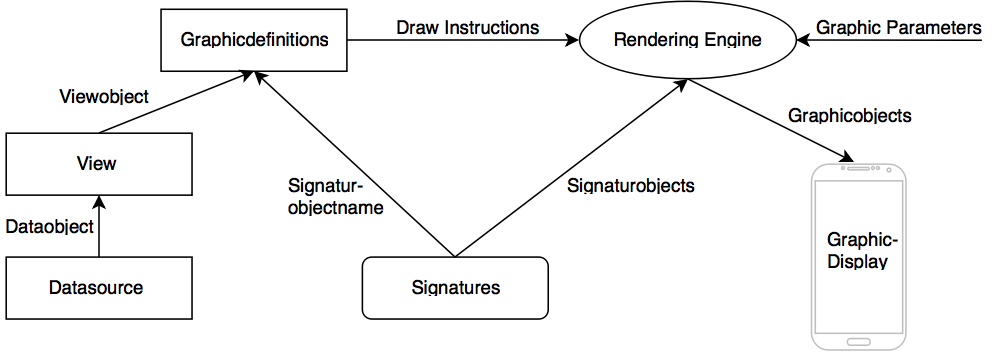
\includegraphics[width=1\textwidth]{images/graphic_definition.png}
  \caption{General graphic definition}
\end{figure}

A layer definition looks like this:
\begin{yamlcode}
- id: landuse
Datasource:
    extent: -20037508.34,-20037508.34,20037508.34,20037508.34
    host: db
    port: 5432
    user: osm
    password: osm
    dbname: osm
    key_field: osm_id
    table: |-
        (
            SELECT osm_id, class, type, geometry
            FROM osm_landusages
            WHERE geometry && !bbox!
            AND z(!scale_denominator!) > 5
        
        ) as data
    type: postgis
fields:
    osm_id: Number
    class: String
    type: String
properties:
    "buffer-size": 4
\end{yamlcode}
The layer definition consist of the id (layername), datasource, fields and the properties. The datasource in this case defines how the postgis database can be accessed and which sql query needs to be executed. But the datasource could also be a geojson, shapefile, sqlite database, geotiff, kml, gpx or csv file.


\subsubsection{Buffers}\label{buffers}
The buffer value on a layer defines how many pixels around each tile will be included. It is necessary to ensure correct rendering across tile boundaries. This value is individual for each layer and depends on the type of data. Buffers for layers containing labels should have a large buffers size such as 128 pixels, whereas a layer like landuse does only need a buffers size of 4 pixels. In general, the buffer size should be set to the minimum to keep the size of the vector tiles as low as possible.\footnote{\url{https://www.mapbox.com/help/source-manual/\#buffers}}

\begin{figure}[h]
  \centering
  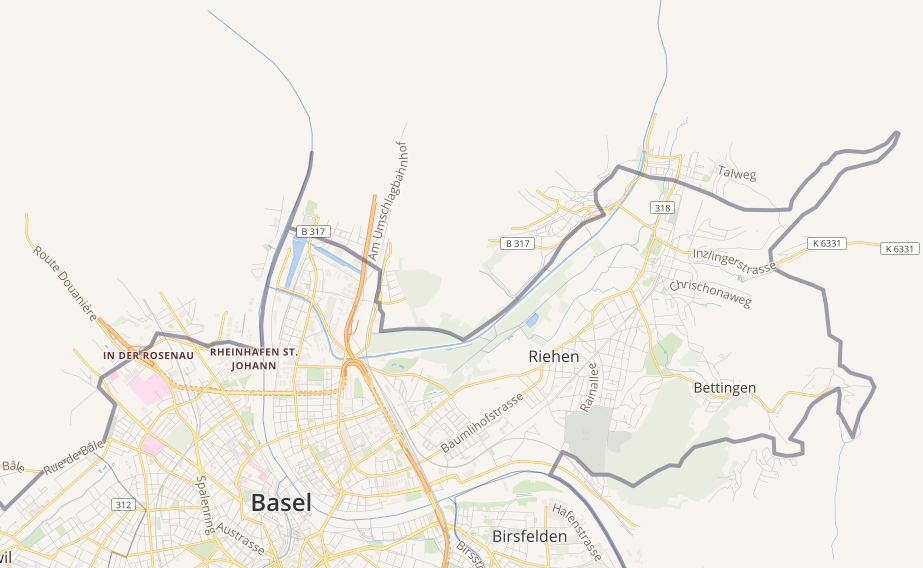
\includegraphics[width=1\textwidth]{images/buffer.png}
  \caption{Example for buffer values}
\end{figure}

The figure above is a good example to see the result of a buffer value. We can see that there are rivers but no other data, therefore the rivers must have a larger buffer value that the other layers.

\subsubsection{Overzooming}\label{overzooming}
The min- and maxzoom values define on which zoom levels there is data. This does not mean that it is not possible to zoom deeper in that the maxzoom value.
Overzooming defines to term of displaying data at higher zoom levels.\footnote{\url{https://www.mapbox.com/help/source-manual/\#overzooming}}
This allows us to show data on higher zoom levels, without generating vector tiles for these zoom levels.
Mapbox has defined a rule of thumb for vector tiles. Vector tiles are useful for about 4-6 levels of overzooming. If I have a vector tile on zoom level 10, it can be stretched out up to zoom level 14 or 16.  

\subsubsection{Layer Ordering}\label{layer_ordering}
The order in which the layer are defined in the data style is equal to the order they are stored in the vector tiles.
The layer at the top of the layer definition will be drawn first next the second layer and so one. So the layer at the bottom is drawn on top of all the other layers. 


\section{Zoom Level Reference}\label{zoomlevel_reference}
The zoom level reference helps to see which feature class is included on which zoom level. The zoom levels are ordered by how they get drawn. The feature class landuse is at the bottom and housenum\_label is on top of all the others. 

% Please add the following required packages to your document preamble:
% \usepackage{graphicx}
\begin{table}[H]
\centering
\resizebox{\textwidth}{!}{%
\begin{tabular}{l|ccccccccccccccc}
 & \multicolumn{1}{l}{z0} & \multicolumn{1}{l}{z1} & \multicolumn{1}{l}{z2} & \multicolumn{1}{l}{z3} & \multicolumn{1}{l}{z4} & \multicolumn{1}{l}{z5} & \multicolumn{1}{l}{z6} & \multicolumn{1}{l}{z7} & \multicolumn{1}{l}{z8} & \multicolumn{1}{l}{z9} & \multicolumn{1}{l}{z10} & \multicolumn{1}{l}{z11} & \multicolumn{1}{l}{z12} & \multicolumn{1}{l}{z13} & \multicolumn{1}{l}{z14} \\ \hline
landuse &  &  &  &  &  & x & x & x & x & x & x & x & x & x & x \\
waterway &  &  &  &  &  &  &  &  & x & x & x & x & x & x & x \\
water & x & x & x & x & x & x & x & x & x & x & x & x & x & x & x \\
aeroway &  &  &  &  &  &  &  &  &  &  &  &  & x & x & x \\
barrier\_line &  &  &  &  &  &  &  &  &  &  &  &  &  &  & x \\
building &  &  &  &  &  &  &  &  &  &  &  &  &  & x & x \\
landuse\_overlay &  &  &  &  &  &  &  & x & x & x & x & x & x & x & x \\
tunnel &  &  &  &  &  &  &  &  &  &  &  & x & x & x & x \\
road &  &  &  &  &  & x & x & x & x & x & x & x & x & x & x \\
bridge &  &  &  &  &  &  &  &  &  &  &  &  & x & x & x \\
admin & x & x & x & x & x & x & x & x & x & x & x & x & x & x & x \\
country\_label &  & x & x & x & x & x & x & x & x & x & x & x & x & x & x \\
marine\_label &  & x & x & x & x & x & x & x & x & x & x & x & x & x & x \\
state\_label &  &  &  &  & x & x & x & x & x & x & x & x & x & x & x \\
place\_label &  &  &  &  & x & x & x & x & x & x & x & x & x & x & x \\
water\_label &  &  &  &  &  &  &  &  &  &  & x & x & x & x & x \\
poi\_label &  &  &  &  &  &  &  &  &  &  &  &  &  &  & x \\
road\_label &  &  &  &  &  &  &  &  & x & x & x & x & x & x & x \\
waterway\_label &  &  &  &  &  &  &  &  & x & x & x & x & x & x & x \\
housenum\_label &  &  &  &  &  &  &  &  &  &  &  &  &  &  & x
\end{tabular}
}
\caption{Shows which feature class is included on which zoom level}
\label{my-label}
\end{table}

\section{Reverse Engineering Process}\label{reverse_engineering_process}
One of the main requirements of this project was to make our vector tiles compatible with the Mapbox Streets vector tiles\footnote{\url{https://www.mapbox.com/developers/vector-tiles/mapbox-streets-v6/}}.

We didn't define this requirement from the beginning, it just evolved during the construction of our first prototype.
Therefore we spent a lot of time making our vector tiles as similar as possible to the ones of Mapbox.

The sections below describe the tools and methods we used to achieve the goal of Mapbox Streets compatibility.

\subsection{Vector Tile Format}\label{vector_tile_format}
To better understand what the vector tile compare tool does, we will give a high level introduction to the vector tiles format.

A vector tile can consist of one or more named layers and containing one or more features. A feature consist of attributes and a geometry (point, linestring or polygon). Attributes are represented as a dictionary of key, value pairs. 

Below you can find an example vector tile, which has two layers water and admin. The water layer has the attribute key "osm\_id" and value 0. If you would compare this example with the specification\footnote{\url{https://github.com/mapbox/vector-tile-spec/tree/master/1.0.1}}, one could think this is not a specification conform vector tile. The example below is a compressed vector tile. More information on what compression methods are applied can be found in the specification. 

Mapbox Streets v6 vector tile(0/0/0):
\begin{jsoncode}
{ 
  "layers": {
    "water": {
      "version": 1,
      "name": "water",
      "extent": 4096,
      "length": 18,
      "_pbf": {
        "buf": [26,143,32,10,5,119,97,1],
        "pos": 51410,
        "length": 51410
      },
      "_keys": ["osm_id"],
      "_values": [0],
      "_features": [11,3474,3499,3530,3561,3584] 
    },
    "admin": {
      "version": 1,
      "name": "admin",
      "extent": 4096,
      "length": 1447,
      "_pbf": {
        "buf": [26,143,32,10,5,1],
        "pos":51410,
        "length":51410
       },
      "_keys": ["admin_level","disputed","iso_3166_1","maritime"],
      "_values": [2,0,"FR",1],
      "_features": [4126,4152,4377,4403,4429,4455,4481,4507,4533]
    }
  } 
}
\end{jsoncode}

\subsection{Tools}\label{tools}
During the prototyping phase we realized, that we needed build tools which help us track the progress of compatibility.

\subsubsection{Vector Tile Compare}\label{vector_tile_compare}
The vector tile compare tool analyzes vector tiles and outputs interesting information like layers and attributes. We generated this output for the same vector tiles of Mapbox Streets and our own (Open Streets). Next we uploaded the results to a Github repository and used the branch compare feature to compare them. 

\begin{figure}[H]
  \centering
  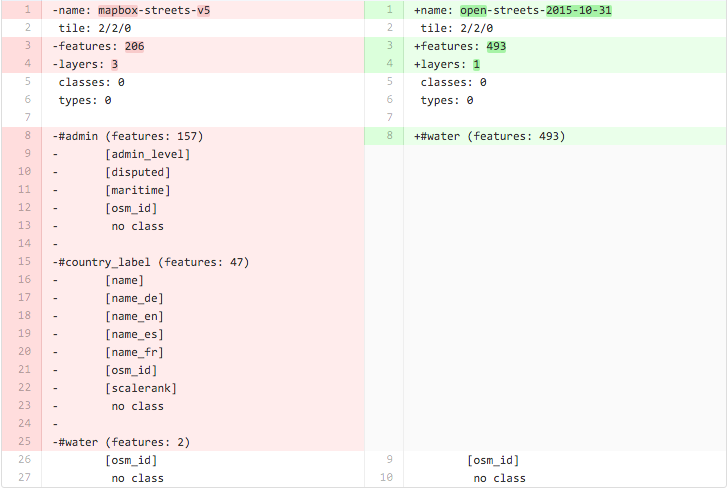
\includegraphics[width=1\textwidth]{images/vector_tile_compare.png}
  \caption{Compare of Mapbox Streets v6 and Open Streets on 31.10.2015}
\end{figure}

This gave us a good indicator, which layers are shown on which zoom level and what attributes are contained in a layer.
\subsubsection{Visual Compare}\label{visual_compare}
The vector tile comparison was good to ensure that we have exactly the same data on the same zoom level. But when we started to visually compare our map with the map of Mapbox Streets, we still saw big differences. So we decided to build a visual compare tool. 

\begin{figure}[H]
  \centering
  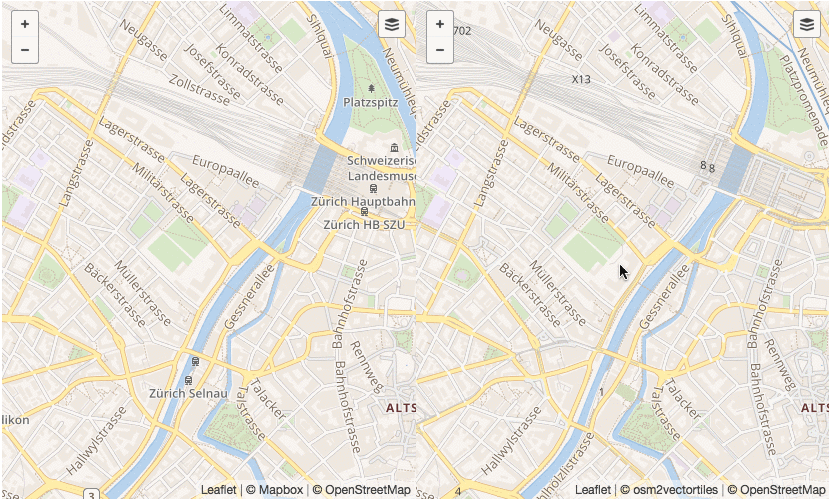
\includegraphics[width=1\textwidth]{images/visual_compare.png}
  \caption{Visual Compare of Mapbox Streets and Open Streets}
\end{figure}

The figure below shows a screenshot of the visual compare tool. On the left side is Mapbox Streets and on the right side our Open Streets map. They both use the same visual style (OSM Bright 2\footnote{\url{https://github.com/mapbox/mapbox-studio-osm-bright.tm2}}). When you zoom in on the right side of the map, it automatically zooms in on the right side. This tools was very helpful to find all the differences.

\subsection{Working Methods}
This section describes what we did, when we found a difference. When we identified a difference with the vector compare or visual compare tool, we first checked if the missing data is included in our import mapping. If this was not the case, we used the TagFinder tool\footnote{\url{https://wiki.openstreetmap.org/wiki/TagFinder}} find the right OSM key, value pair of the missing item. Next we included the key, value pair into our import mapping and re-imported the OSM data. At the end the SQL query needs to be altered to fetch the added item. Now the missing item should appear on the map. During this process we used mostly Mapbox Studio Classic\footnote{\url{https://www.mapbox.com/mapbox-studio-classic/}} as the map can be rendered on the fly after the query has been altered.

\section{Data Sources}
\label{data-sources}

Making a global map involves finding the right data slice in the right data sources.

\subsection{Map Features from OpenStreetMap}

The cornerstone of the entire map is \osm data from published snapshots from OSM Planet\footnote{\url{http://planet.osm.org/}}. The \osm{} data is used for high zoom levels where detailled coverage of local areas is very important.

We import selected tags \footnote{\url{http://wiki.openstreetmap.org/wiki/Tags}} and their geometries. The decision which tags and geometries are imported is in the chapter mapping

TODO: Create label for mapping

\subsection{Curated water polygons from OpenStreetMapData}

Certain OpenStreetMap data like borders and land polygons are very sensitive for change.
The OpenStreetMapData\footnote{\url{http://openstreetmapdata.com/}}
project takes care of alot of issues that happen with coastlines
and provide it in a convenient format.

We use water polygons \footnote{\url{http://openstreetmapdata.com/data/water-polygons}} from OpenStreetMapData. This data set ensures that the water polygons
work well together with other \osm{} data and splits big water polygons into multiple 
pieces for performance.

\section{Borders and ranks from Natural Earth}

The Natural Earth \footnote{\url{http://www.naturalearthdata.com/}} dataset provides manually curated data of cultural and physical features of the world. Natural earth data is especially useful at higher levels when it matters alot what should not be displayed.

We use the following data from Natural Earth:

\begin{itemize}
\item Label ranks of big cities\footnote{\url{http://www.naturalearthdata.com/downloads/10m-cultural-vectors/10m-populated-places/}}
\item Major lakes\footnote{\url{http://www.naturalearthdata.com/downloads/10m-physical-vectors/10m-lakes/}}
\item Country\footnote{\url{http://www.naturalearthdata.com/downloads/10m-cultural-vectors/10m-admin-0-countries/}} and administrative\footnote{\url{http://www.naturalearthdata.com/downloads/10m-cultural-vectors/10m-admin-1-states-provinces/}} borders including disputed borders\footnote{\url{http://www.naturalearthdata.com/downloads/10m-cultural-vectors/10m-admin-0-breakaway-disputed-areas/}}
\end{itemize}


\section{PostgreSQL Performance}
\label{postgres-performance}

The most intensive work is done on the database side to respond to all SQL queries
made by Mapnik in the fastest way possible.

\subsection{Tuning}

The PostgreSQL default parameters do not deliver good performance for stronger machines\footnote{\url{https://wiki.postgresql.org/wiki/Tuning_Your_PostgreSQL_Server}-}
For the different database machines we used the PgTune\footnote{\url{http://pgtune.leopard.in.ua/}} calculator to determine good cache and buffer sizes for data warehouse style computing.

Example configuration for a host with 50 GB of memory.

\begin{bashcode}
max_connections = 20
shared_buffers = 12800MB
effective_cache_size = 38400MB
work_mem = 320MB
maintenance_work_mem = 2GB
checkpoint_segments = 128
checkpoint_completion_target = 0.9
wal_buffers = 16MB
default_statistics_target = 500
\end{bashcode}

For speed up importing we disabled transactional features of PostgreSQL. \footnote{\url{http://www.databasesoup.com/2015/02/running-with-scissors-mode.html}}.

\begin{bashcode}
bgwriter_lru_maxpages = 0
wal_level = minimal
fsync = off
synchronous_commit = off
full_page_writes = off
wal_log_hints = off
\end{bashcode}


\subsection{Indizes}

We use clustered indizes on the geometries to provide fast tile lookup.\newpage
\chapter{Results and Future}\label{part2_results_and_future}

\section{Results}\label{part2_results}
The result of this study thesis are described in Part 1, \hyperref[part1_results]{\emph{section 4.1}}.

\section{Future Development}\label{part2_future_development}
The first version of our vector tiles have shown, that it is possible to get very close to compatibility with Mapbox Streets in a reasonable amount of time. There are still some quirks, which needs to be ironed out but we created a good foundation for future development. The two sections below describe small improvements and new features which will be implemented in our bachelor thesis.

\subsection{Small improvements}\label{small_improvements}
 
\paragraph{Labels}
The scalerank of the place, marine, state and road labels should be improved. Our current implementation is alright for the moment, but still not equal to Mapbox Street.

\paragraph{State Labels}
State labels are used to display states of big countries like USA, Russia or China. More state labels could be added. 

\paragraph{Country boundaries}
At the moment we use a mix of Natural Earth and OSM data for the administrative boundaries. We had to implement this layer with data of both data sources, because we had some graphical issues with the OSM data on small zoom levels. Using Natural Earth data alone is not suitable, because the data is generalized. Therefore it does not look good on high zoom levels.

\paragraph{Country Name Translation Rule}
Mapbox has defined a fallback rule\footnote{\url{https://www.mapbox.com/developers/vector-tiles/mapbox-streets-v6/}} for the country names. We struggled implementing it and had to prioritize on other features.

\paragraph{Special Maki Icons for US Road Labels}
Mapbox uses different maki icons\footnote{\url{https://www.mapbox.com/maki/}} for the road labels in the US.  

\paragraph{Possiblity of Mapbox Terrain Visual Style}
Check if all the data required for a Mapbox style like Mapbox Rerrain\footnote{\url{https://www.mapbox.com/developers/vector-tiles/mapbox-terrain/}} is included in our vector tiles

\paragraph{Exclude Water in Rendering Process}
When we implemented the vector tile rendering process, we realized that a lot of rendering time could be saved when the water (no data) is excluded. It turned out, that deciding if a vector tiles will have no data, is not an easy problem. So we just render everything and remove the "empty" vector tiles afterwards.  

\subsection{New Features}\label{new_features}

\paragraph{Vector Tiles of Entire World}
One of the main targets of our bachelor thesis is to render the vector tiles of the entire world. This brings new challenges like scaling our rendering infrastructure. 

\paragraph{Update Vector Tiles}
A big request of the Swiss OSM community was to provide updated vector tiles based on the diff\footnote{\url{http://wiki.openstreetmap.org/wiki/Planet.osm/diffs}} files.

\paragraph{Faster Tile Server}
During our research of existing vector tile servers we found out, that there is no robust, scalable vector tile server available. This could maybe even be a separate project.

\paragraph{GeoName Search}
If we want to fulfill the long term goal of this project to provide an offline map, we should definitly implement basic GeoName search capability.

\newpage{}\newpage
\chapter{Project Management}\label{project-management}

\section{Milestones}

\paragraph{START}
Getting familiar with tools and topic.

\paragraph{ALPHA}
Create a proof of concept tileserver.

\paragraph{BETA}
Rendering switzerland.

\paragraph{PREFINAL}
Good looking lower tiles.

\paragraph{FINAL}
Rendering.

\section{Releases}

\paragraph{v0.1 BETA}
Tooling of entire workflow to render switzerland.

\paragraph{v0.2 PREFINAL}
Used for initial rendering.

\paragraph{v1 FINAL}
Included lessons learned from v0.2

\section{Roles and Responsibilities}\label{roles-and-responsibilities}

\paragraph{Stefan Keller}
Thesis advisor responsible for supervising the work.

\paragraph{Petr Pridal}
Technical partner responsible for providing infrastructure and guidance
in technical and map relatec questions.

\paragraph{Manuel Roth}
Contributor responsible for data style and JavaScript tooling.

\paragraph{Lukas Martinelli}
Contributor responsible for rendering infrastructure and Python scripts.

\section{Aufwandschätzung, Zeitplan, Projektplan}

\section{Risks}\label{risks}

\section{Prozessmodell}

We used GitHub for planning and tracking the tasks.

Our sprints are organized into milestones and tasks were assigned to a milestone

Managing tickets, milestones and progress all happens on the public
GitHub repository.



There are two GitHub repositories:

\begin{itemize}
\item
  \textbf{osm2vectortile} contains the project
\item
  \textbf{osm2vectortile-thesis} contains the thesis
\end{itemize}

%---------------------------------------------------------------
\newpage
\chapter{Quality Measures}\label{quality-measures}

\section{Testing}\label{testing}

Our ecosystem is quite a diverse one with a big collection of small
tools that all work together. Therefore we use high level integration
tests to ensure that our components work together.

TODO: How did we test? Visual compare already explains a bit.

\section{Guidelines}\label{guidelines}
To have a homogenous software we settled on common guidelines in 
the beginning of the project.

\subsection{Releases}
We use semantic versioning \footnote{\url{http://semver.org/}}. At the
end of each milestone a new release will be created.

\subsection{Git}\label{git}
\paragraph{Commit Messages}
We use the seven rules of great git commit
messages\footnote{\url{http://chris.beams.io/posts/git-commit/}}.

\paragraph{Rewriting}
Git history should be kept clean and therefore local branches should be
squashed meaningfully.

\paragraph{Pulling}
To avoid unnecessary merge messages one should always use the
\texttt{-\/-rebase} parameter.

\subsection{Workflow}\label{workflow}
We use the Feature Branch Workflow\footnote{\url{https://www.atlassian.com/git/tutorials/comparing-workflows/feature-branch-workflow/}}.

Every project member has a local repository with a copy of the remote
repository. For each feature ticket in GitHub a separate branch
will be created. Once a ticket has been completed a pull request will be
created and needs to be merged into the \texttt{master} branch by an other 

\subsection{Coding Standards}

\paragraph{Bash} We use Bash for our Docker image entrypoints and follow
the rules of Defensive Bash Programming \footnote{\url{http://www.kfirlavi.com/blog/2012/11/14/defensive-bash-programming/}}.

\paragraph{Python} For Python code we want to stay PEP-8\footnote{\url{https://www.python.org/dev/peps/pep-0008/}} compliant and write idiomatic Python code according to PEP-20\footnote{\url{https://www.python.org/dev/peps/pep-0020/}}.

\paragraph{JavaScript}


\paragraph{SQL} Our PostgreSQL code is using upper case for the key words. Apart from that we try to have nice formatted SQL code and use functions
if necessary to keep the queries DRY\footnote{\url{https://en.wikipedia.org/w/index.php?title=Don%27t_repeat_yourself&oldid=691047461}}.

\paragraph{Dockerfile} Dockerfiles follow the best practices\footnote{\url{https://docs.docker.com/engine/articles/dockerfile\_best-practices/}} defined by Docker.

%---------------------------------------------------------------\newpage
\newpage
\chapter{Project Monitoring}\label{project monitoring}


\section{Estimated Time vs Actual Time}

Our estimations were too optimistic. Due to the extensive
training period required to get started in a GIS environment
the actual time was more than originally estimated.


\begin{center}
    \begin{tabular}{lll}
    \hline
    Calendar Week & Actual & Estimated    \\
    \hline
    38     & 23:42:33         & 18:35:33          \\
    39     & 32:45:01         & 31:34:03          \\
    40     & 11:17:25         & 12:05:11          \\
    41     & 38:09:20         & 34:35:47          \\
    42     & 33:20:09         & 32:54:22          \\
    43     & 39:04:39         & 38:32:57          \\
    44     & 61:33:10         & 56:40:56          \\
    45     & 52:45:09         & 45:54:43          \\
    46     & 44:22:18         & 41:35:12          \\
    47     & 31:40:00         & 31:21:12          \\
    48     & 11:13:00         & 13:32:42          \\
    \hline
    Total & 379:52:44        & 357:22:38         \\
    \end{tabular}
\end{center}

\section{Time per Person}

Both contributors invested about the same amount of time.

\begin{center}
    \begin{tabular}{llll}
    \hline
     Calendar Week & Lukas Martinelli & Manuel Roth & Total    \\
    \hline
    38     & 13:22:06         & 10:20:27    & 23:42:33  \\
    39     & 16:20:01         & 16:25:00    & 32:45:01  \\
    40     & 2:25:00          & 8:52:25     & 11:17:25  \\
    41     & 20:09:20         & 18:00:00    & 38:09:20  \\
    42     & 22:20:09         & 11:00:00    & 33:20:09  \\
    43     & 10:34:39         & 28:30:00    & 39:04:39  \\
    44     & 30:33:10         & 31:00:00    & 61:33:10  \\
    45     & 27:15:09         & 25:30:00    & 52:45:09  \\
    46     & 18:22:18         & 26:00:00    & 44:22:18  \\
    47     & 15:40:00         & 16:00:00    & 31:40:00  \\
    48     & 7:13:00          & 4:00:00     & 11:13:00  \\
    \hline
    Total & 184:14:52        & 195:37:52   & 379:52:44 \\
    \end{tabular}
\end{center}

\newpage\newpage

%------------------------------------------------
\newpage
\part{Software Documentation}
\chapter{User Documentation}

\section{Display a Raster Map}

This tutorial describes how to get a raster tile map with OSM Vector
Tiles as data source.

\subsection{Result}

You get a basic raster tile map similar to the map below.

\hypertarget{osm-bright-map}{}

\subsection{Preparation}

\begin{enumerate}
\item
  \href{http://osm2vectortiles.org/data/download.html}{Download} an
  extract you want to serve.
\item
  \href{https://github.com/mapbox/mapbox-studio-osm-bright.tm2.git}{Download}
  the visual style.
\item
  Add both to the same directory and make sure that the have the same
  name
\end{enumerate}

\subsection{Install Kitematic}

\begin{enumerate}
\item
  \href{https://www.docker.com/docker-toolbox}{Download} and install
  Kitematic.
\item
  Start a new container by searching for \texttt{osm2vectortiles} and
  click create on the container called \texttt{serve}.
\end{enumerate}

\begin{figure}[H]
\centering
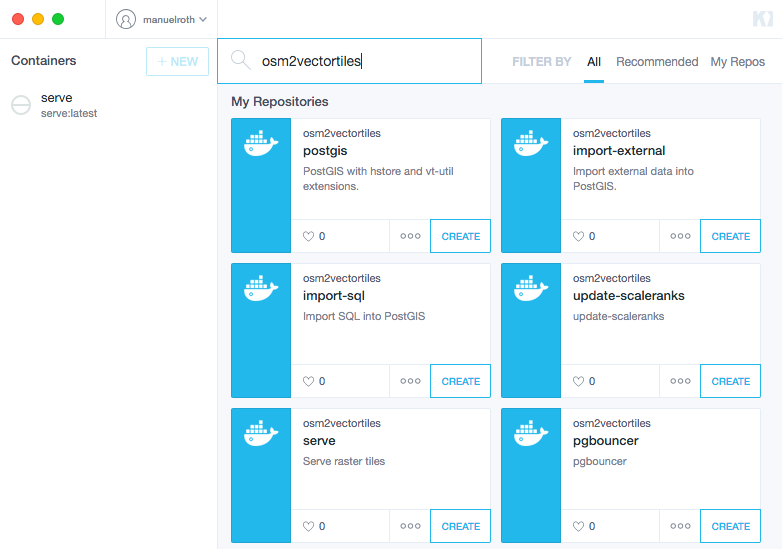
\includegraphics[width=1\textwidth]{images/search_container.png}
\caption{Search Container}
\end{figure}

\subsection{Kitematic Usage}\label{kitematic-usage}

When you start the container, it will complain about missing
\texttt{tm2} style projects.

\begin{figure}[H]
\centering

\includegraphics[width=1\textwidth]{images/tileserver_kitematic_started.png}
\caption{Container started unsucessfully}
\end{figure}

Mount your the directory containing the \texttt{mbtiles} files and
\texttt{tm2} style projects into the \texttt{/data} volume.

\begin{figure}[H]
\centering
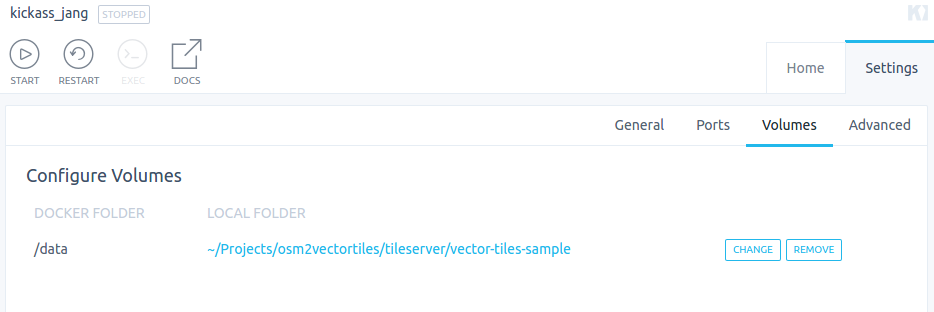
\includegraphics[width=1\textwidth]{images/tileserver_kitematic_volumes_configured.png}
\caption{Configured volumes for container}
\end{figure}

Now restart the container. You should be up and running serving
generated raster tiles.

\begin{figure}[H]
\centering
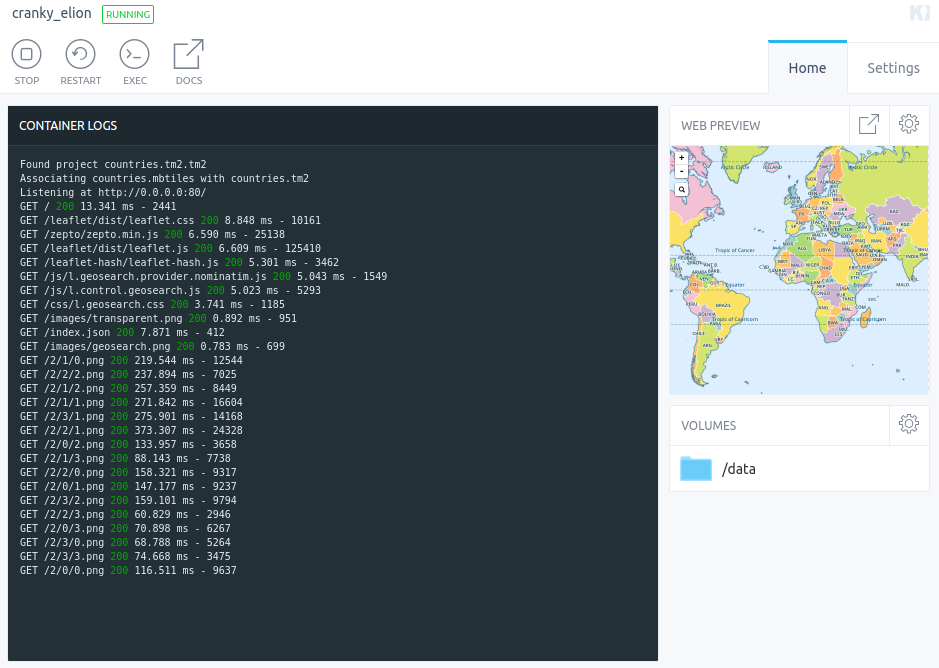
\includegraphics[width=1\textwidth]{images/tileserver_kitematic_running.png}
\caption{Container running and serving tiles}
\end{figure}

%-------------------------------
\section{Display Map with MapboxGL}\label{display-map-with-mapboxgl}

To display a custom MapboxGL based map you need to create a HTML file
and reference the public vector tile server of osm2vectortiles. You are
free to download and host the vector tiles yourself but we provide a
fast and distributed CDN service for serving the PBFs for you.

The easiest way to get started is using the
\texttt{mapbox-gl-js-exmaple} repository. Clone the repository and
change into the directory.

\begin{bashcode}
git clone https://github.com/osm2vectortiles/mapbox-gl-js-example.git
\end{bashcode}

\subsection{Configure Source, Fonts and
Sprites}\label{configure-source-fonts-and-sprites}

In order for Mapbox GL JS to work you also need to provide the
\href{https://www.mapbox.com/mapbox-gl-style-spec/\#glyphs}{fonts} and
\href{https://www.mapbox.com/mapbox-gl-style-spec/\#sprite}{sprites}.
These resources are contained in the folder \texttt{assets}.

The \href{https://www.mapbox.com/mapbox-gl-style-spec/}{Mapbox GL Style
JSON} of OSM Bright is located at \texttt{bright-v8.json}. You can
create your own styles with Mapbox Studio.

If you want to serve the Mapbox GL Style JSON without Mapbox you need to
configure three URLs.

\begin{enumerate}
\item
  Change the \texttt{sources} URL to the free osm2vectortile serve or
  use your own server
\item
  Change the \texttt{sprite} URL to the location of your sprites
\item
  Change the \texttt{glyphs} URL to the location of your fonts
\end{enumerate}

\begin{javascriptcode}
"sources": {
    "mapbox": {
        "url": "http://vectortiles.osm2vectortiles.org/world.json",
        "type": "vector"
    }
},
"sprite": "/assets/sprite",
"glyphs": "/assets/font/{fontstack}/{range}.pbf"
\end{javascriptcode}

\subsection{Initialize the Map}\label{initialize-the-map}

In order to serve a MapboxGL based map you need a
\href{https://www.mapbox.com/mapbox-gl-style-spec/}{Mapbox GL style
JSON} created with \href{https://www.mapbox.com/mapbox-studio/}{Mapbox
Studio}. In this example we will serve the free OSM Bright style
\href{https://github.com/mapbox/mapbox-gl-styles}{provided by Mapbox}.

The HTML file defines a full screen map and the CSS and JavaScript files
required by Mapbox GL JS. The \texttt{bright-v8.json} style is loaded
from the local directory.

Because we use the local sprites and fonts we don't need a Mapbox API
key.

\begin{htmlcode}
<!DOCTYPE html>
<html>
<head>
    <meta charset='utf-8' />
    <title>MapBox GL JS with osm2vectortiles Example</title>
    <meta name='viewport' content='initial-scale=1,maximum-scale=1,user-scalable=no' />
    <script src='//api.tiles.mapbox.com/mapbox-gl-js/v0.10.0/mapbox-gl.js'></script>
    <link href='//api.tiles.mapbox.com/mapbox-gl-js/v0.10.0/mapbox-gl.css' rel='stylesheet' />
    <style>
        body { margin:0; padding:0; }
        #map { position:absolute; top:0; bottom:0; width:100%; }
    </style>
</head>
<body>

<div id='map'></div>
<script>
mapboxgl.accessToken = 'NOT-REQUIRED-WITH-YOUR-VECTOR-TILES-DATA';

var map = new mapboxgl.Map({
    container: 'map',
    style: '/bright-v8.json',
    center: [8.3221, 46.5928],
    zoom: 1,
    hash: true
});
map.addControl(new mapboxgl.Navigation());
</script>
</body>
</html>
\end{htmlcode}


\subsection{Serve the Map}

You need a simple HTTP server for serving the HTML and

%-------------------------------

%-------------------------------

\section{Create a new Style with Mapbox Studio
Classic}\label{create-a-new-style-with-mapbox-studio-classic}

You can use
\href{https://www.mapbox.com/help/getting-started-studio/}{the same
resources from Mapbox} for learning how to design maps with Mapbox
Studio Classic. This tutorial will show you how to customize the OSM
Bright style.

Download \href{https://www.mapbox.com/mapbox-studio-classic/}{Mapbox
Studo Classic} to create your first map.

\subsection{Create new style project}\label{create-new-style-project}

Create a new style project based of OSM Bright. You can also start with
a blank slate but it is easier to get started from an existing style.

In \texttt{Styles\ and\ Resources} create a new style and choose
\texttt{OSM\ Bright\ 2}. Then save your project.

\begin{figure}[H]
\centering
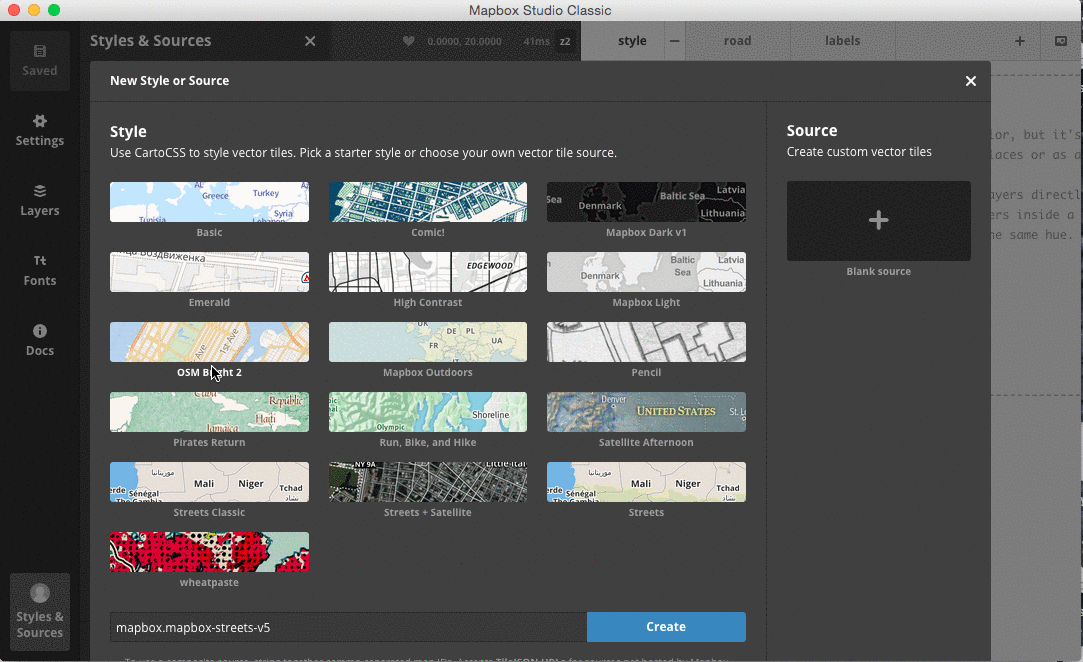
\includegraphics[width=1\textwidth]{images/mapbox_classic_create_project.png}
\caption{Create new project with Mapbox Studio Classic}
\end{figure}

\subsection{Switch to osm2vectortiles}\label{switch-to-osm2vectortiles}

Now you are based of the vector tiles from Mapbox Streets. To use our
free and Open Source vector tiles you need to \texttt{Change\ Source} in
\texttt{Layers}.

Enter the \href{https://github.com/mapbox/tilejson-spec}{TileJSON} url
of our vectortiles server
\texttt{vectortiles.osm2vectortiles.org/world.json}. You can later
replace this with your own vector tiles server if you want to serve
everything by yourself.

Because our vector tiles are to a large part Mapbox Streets compatible
you won't see any drastic changes. In fact you could even continue
styling your project with Mapbox Streets and make the switch at the
deployment stage of the project.

\begin{figure}[htbp]
\centering
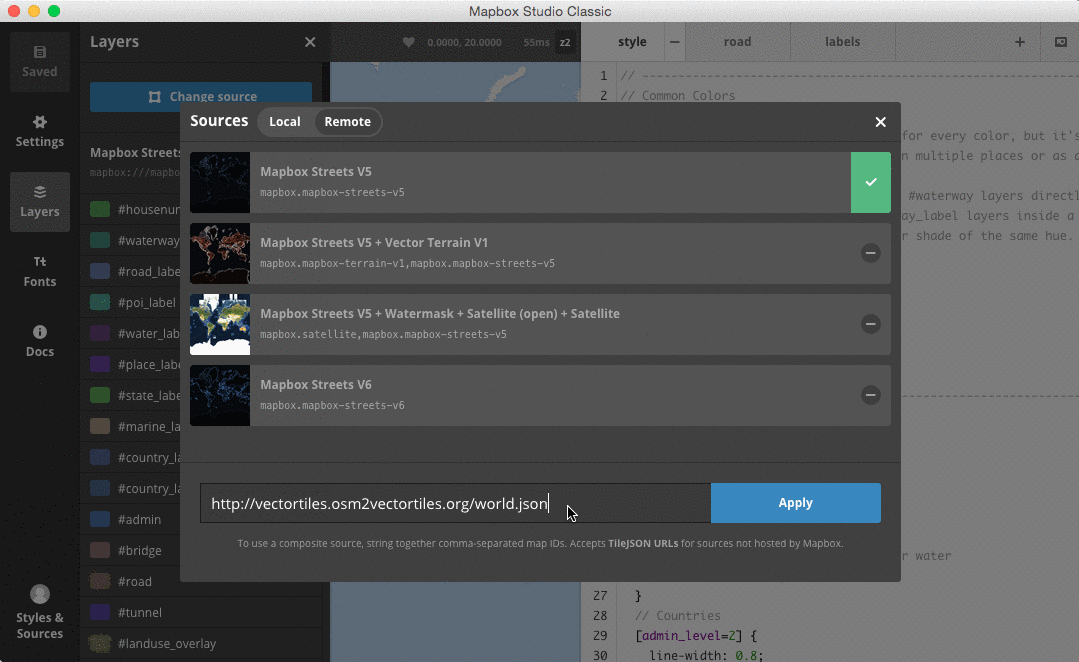
\includegraphics[width=1\textwidth]{images/mapbox_classic_switch_osm2vectortiles.png}
\caption{Switch to osm2vectortiles in Mapbox Studio Classic}
\end{figure}

\subsection{Deploy your Map}\label{deploy-your-map}

Because you are no longer bound to Mapbox for hosting you can now host
the maps yourself and save money.

%-------------------------------

\section{Create a new Style with new Mapbox
Studio}\label{create-a-new-style-with-new-mapbox-studio}

Mapbox Studio is the new Map design platform by Mapbox. Mapbox provides
\href{https://www.mapbox.com/help/getting-started-mapbox-studio-1/}{great
resources for getting started} how to design your own maps. This
tutorial will show you how to customize the OSM Bright style for Mapbox
GL.

Visit \href{https://www.mapbox.com/studio/}{the Mapbox Studio Editor}
and follow the tutorial.

\subsection{Create new style project}\label{create-new-style-project}

Create a new style project. Make sure you start of a base map that only
requires Mapbox Streets. A Mapbox Terrain equivalent is not available by
osm2vectortiles.

In \texttt{Styles} create a new style, choose \texttt{Bright} and save
your project.

\begin{figure}[H]
\centering
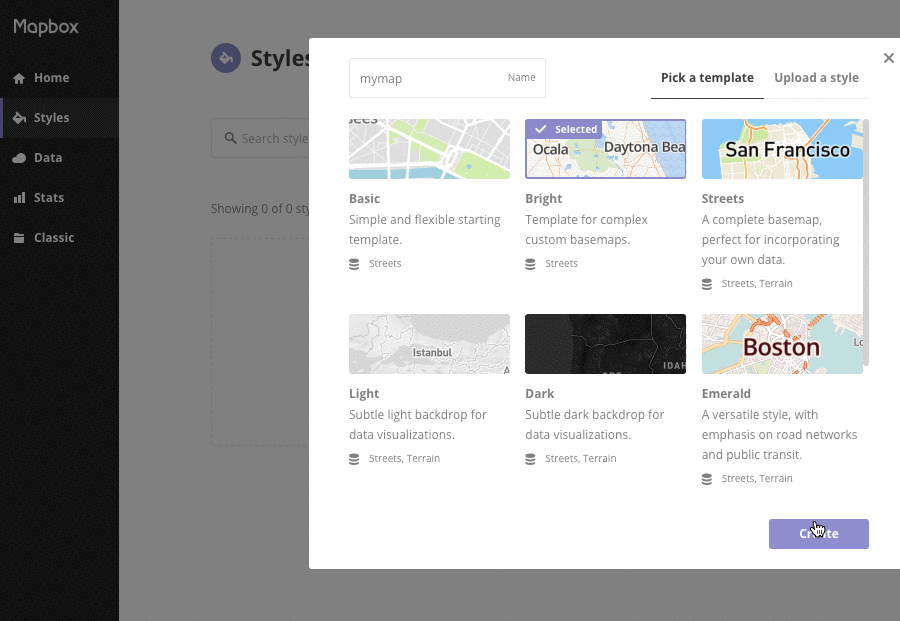
\includegraphics[width=1\textwidth]{images/mapbox_studio_create_style.png}
\caption{Create new project with new Mapbox Studio}
\end{figure}

\subsection{Switch to osm2vectortiles}\label{switch-to-osm2vectortiles}

In the new Mapbox Studio you can no longer specify a
\href{https://github.com/mapbox/tilejson-spec}{TileJSON} url of a custom
vectortiles server. Therefore it is best to work with the original
Mapbox Streets v6 data in the editor and make the switch to
osm2vectortiles at the deployment step. This works because our vector
tiles are to a large part Mapbox Streets v6 compatible.

Because users have an upload limit for their own data sources you cannot
upload the osm2vectortiles world file to Mapbox Studio and style it
directly. However if you want to work with the real data you can choose
an extract which is quite small (below 100MB) and upload it to Mapbox
Studio and work on this sample extract to create your map.
\chapter{Developer Documentation}

\section*{Create your own vector tiles}

Docker is used extensively for development and deployment. The easiest
way to get started is using
Docker Compose\footnote{\url{https://www.docker.com/docker-compose}}.
\\\\
1. Step: Clone the osm2vectortiles project.

\begin{bashcode}
git clone https://github.com/osm2vectortiles/osm2vectortiles.git
\end{bashcode}

2. Step: Start up your PostGIS container with the data container attached.

\begin{bashcode}
docker-compose up -d postgis
\end{bashcode}

3. Step: Download a PBF and put it into the local \texttt{import} directory.

\begin{bashcode}
wget https://s3.amazonaws.com/metro-extracts.mapzen.com/zurich_switzerland.osm.pbf
\end{bashcode}

4. Step: Now you need to import the PBF files into PostGIS.

\begin{bashcode}
docker-compose up import-osm
\end{bashcode}

5. Step: Now you need to import several external data sources.

Import water polygons from OpenStreetMapData.

\begin{bashcode}
docker-compose up import-water
\end{bashcode}

6. Step: Import Natural Earth data for lower zoom levels.

\begin{bashcode}
docker-compose up import-natural-earth
\end{bashcode}

7. Step: Import custom country, sea and state labels.

\begin{bashcode}
docker-compose up import-labels
\end{bashcode}

8. Step: Now import custom SQL functions.

\begin{bashcode}
docker-compose up import-sql
\end{bashcode}

9. Step: Update the scaleranks of OSM places.

\begin{bashcode}
docker-compose up update-scaleranks
\end{bashcode}

10. Step: Export the data as MBTiles file to the \texttt{export} directory.

\begin{bashcode}
docker-compose up export
\end{bashcode}

11. Step: Serve the tiles as raster tiles from \texttt{export} directory.

\begin{bashcode}
docker-compose up serve
\end{bashcode}



\section*{Create own extract}\label{create-own-extract}

If you need an extract which is not included on the
downloads page\footnote{\url{http://osm2vectortiles.org/data/download.html}},
you can download the planet file and make your own extract.

\subsection*{Preparation}

\begin{enumerate}
\item
  Download\footnote{\url{http://osm2vectortiles.org/data/download.html}} the
  planet file.
\item
  Get the bounding box of your desired extract.\footnote{\url{http://tools.geofabrik.de/calc/\#type=geofabrik_standard\&bbox=5.538062,47.236312,15.371071,54.954937\&tab=1\&proj=EPSG:4326\&places=2}}
\item
  Install tilelive utility.

\begin{bashcode}
npm install -g tilelive
\end{bashcode}
\end{enumerate}

\subsection*{Create Extract}\label{create-extract}

To create an extract the \texttt{tilelive-copy} utility is used. It takes a
bounding box and a MBTiles file as input and ouputs the extract.

Replace the bounding box in the following command with your bounding
box.

\begin{bashcode}
tilelive-copy --minzoom=0 --maxzoom=14 --bounds="60.403889,29.288333,74.989862,38.5899217" 
world.mbtiles switzerland.mbtiles
\end{bashcode}
\newpage

\section*{Layer Reference}\label{layer-reference}

This is a guide to the data inside the OSM Vector Tiles to help you with
styling.

Available layers:

\begin{itemize}
\item
  landuse
\item
  waterway
\item
  water
\item
  aeroway
\item
  barrier\_line
\item
  building
\item
  landuse\_overlay
\item
  tunnel
\item
  road
\item
  bridge
\item
  admin
\item
  country\_label
\item
  marine\_label
\item
  place\_label
\item
  water\_label
\item
  poi\_label
\item
  road\_label
\item
  waterway\_label
\item
  housenum\_label
\end{itemize}

\subsection*{landuse}\label{landuse}

This layer includes polygons representing both land-use and land-cover.

It's common for many different types of landuse/landcover to be
overlapping, so the polygons in this layer are ordered by the area of
their geometries to ensure smaller objects will not be obscured by
larger ones. Pay attention to use of transparency when styling - the
overlapping shapes can cause muddied or unexpected colors.

\subsection*{water}\label{water}

This is a simple polygon layer with no differentiating types or classes.
Water bodies are filtered and simplified according to scale - only
oceans and very large lakes are shown at the lowest zoom levels, while
smaller and smaller lakes and ponds appear as you zoom in.

\subsection*{waterway}\label{waterway}

The waterway layer contains rivers, streams, canals, etc represented as
lines.

\subsubsection*{Type}

The \texttt{type} column can contain one of the following types:

\begin{itemize}
\item
  \texttt{ditch}
\item
  \texttt{stream}
\item
  \texttt{stream\_intermittent}
\item
  \texttt{river}
\item
  \texttt{canal}
\item
  \texttt{drain}
\item
  \texttt{ditch}
\end{itemize}

\subsection*{aeroway}\label{aeroway}

The aeroway layer contains the types runway, taxiway, apron and helipad.

\subsection*{barrier\_line}\label{barrierux5fline}

The barrier\_line layer contains the classes fence, cliff, gate.

\subsection*{building}\label{building}

This layer contains buildings. Buildings are shown starting zoom level
13.

\subsection*{landuse\_overlay}\label{landuseux5foverlay}

This layer is for landuse polygons that should be drawn above the
\#water layer.

\subsection*{tunnel, road, bridge}\label{tunnel-road-bridge}

The layers tunnel and bridge are based of the layer road.

\subsubsection*{Class}

The main field used for styling the tunnel, road, and bridge layers is the \texttt{class} field.

\begin{table}[H]
\label{my-label}
\begin{tabular}{p{3cm} | p{8cm}}
Class           & Aggregated Types                                                                                                              \\ \hline
motorway        & motorway                                                                                                                      \\
motorway\_link  & motorway\_link                                                                                                                \\
driveway        & driveway                                                                                                                      \\
main            & primary, primary\_link, trunk, trunk\_link, secondary, secondary\_link, tertiary, tertiary\_link                              \\
street          & residential, unclassified, living\_street, road, raceway                                                                      \\
street\_limited & pedestrian, construction, private                                                                                             \\
service         & service, track, alley. spur, siding, crossover                                                                                \\
path            & path, cycleway, ski, steps, bridleway, footway                                                                                \\
major\_rail     & rail, monorail, narrow\_gauge, subway                                                                                         \\
aerialway       & chair\_lift, mixed\_lift, drag\_lift, platter, t-bar, magic\_carpet, gondola, cable\_car, rope\_tow, zip\_line, j-bar, canopy \\
golf            & hole                                                                                                                          \\
                &                                                                                                                              
\end{tabular}
\end{table}

\subsection*{admin}

This layer contains the administrative boundary lines. These are based
on Natural Earth data on lower zoom levels (0-6) and OSM data (7-14) on
upper zoom levels.

\subsubsection*{Administrative Levels}

The administrative levels are in the \texttt{admin} field. 

\begin{table}[H]
\label{my-label}
\begin{tabular}{l | l}
Value & Aggregated Types  \\ \hline
2     & countries         \\
4     & states, provinces
\end{tabular}
\end{table}

The \texttt{disputed} field should be used to apply a dashed or otherwise
distinct style to disputed boundaries.

\subsubsection*{Maritime Boundaries}

The \texttt{maritime} field can be used as a filter to downplay or hide maritime
boundaries, which are often not shown on maps.

\subsubsection*{Localrank}

The \texttt{country\_label} layer contains the labels of all countries with
translated names.

\subsubsection*{Localrank}

The \texttt{scalerank} field is used to hide or show the label based on the
importance, size and available room.

\subsection*{marine\_label}\label{marine_label}

The marine\_label layer contains labels for marine features such as
oceans, seas, large lakes and bays.
The \texttt{labelrank} is used to hide or show the label based on the importance,
size and available room.

\subsection*{state\_label}\label{state_label}

The layer state\_label contains labels for large provinces in large
countries such as China, USA, Russia, Australia and UK.

\subsection*{place\_label}\label{place_label}

The layer place\_label contains labels for cities.

\subsubsection*{Scalerank}

The scalerank is used to hide or show the label based on the importance,
size and available room.

\subsubsection*{Localrank}

The \texttt{localrank} field can be used to adjust the label density by showing
fewer labels.

\subsection*{water\_label}

The layer water\_label contains labels for bodies of water such as
lakes.

\subsection*{road\_label}

The layer road\_label uses the same classification as the layer road.

\subsection*{waterway\_label}

The layer waterway\_label contains labels for rivers.

\subsection*{housenum\_label}

This layer contains points used to label the street number parts of
specific addresses. Both housenumber polygons and points were mapped to
a single layer.
The \texttt{house\_num} field countains house and building numbers.

\subsection*{poi\_label}

The poi\_label layer is used to place icons and labels for various point
of interests.

\subsubsection*{Names}

Names are available in all languages (name, name\_en, name\_de,
name\_fr, name\_es, name\_ru, name\_zh).

\subsubsection*{Scalerank}

The scalerank of a POI is determined by the area.

\begin{table}[H]
\label{my-label}
\begin{tabular}{l | l}
Scalerank & Description                                       \\ \hline
1         & The POI has a very large area \textgreater145000  \\
2         & The POI has a medium-large area \textgreater12780 \\
3         & The POI has a small area 2960 or is a station     \\
4         & The POI has no known area                        
\end{tabular}
\end{table}

\subsubsection*{Localrank}

The localrank field can be used to adjust the label density by showing
fewer labels. The localrank is a whole number which starts at 1 and
groups places in a grid by their importance.

Importance of POIs are weighted in the following order:

\begin{enumerate}
\def\labelenumi{\arabic{enumi}.}
\item
  station, subway\_entrance, park, cemetery, bank, supermarket, car,
  library, university, college, police, townhall, courthouse
\item
  nature\_reserve, garden, public\_building
\item
  stadium
\item
  hospital
\item
  zoo
\item
  university, school, college, kindergarten
\item
  supermarket, department\_store
\item
  nature\_reserve, swimming\_area
\item
  attraction
\end{enumerate}

\subsubsection*{Maki Labels and Types}\label{maki-labels-and-types}

The \texttt{type} field in the poi\_label layer is mapped to the appropriate Maki
label which can be queried in maki. Types are stored in a human readable
format in the data where chair\_lift becomes Chair lift so you can use
the type field for as label.


%------------------------------------------------
%	THESIS CONTENT - APPENDICES
%------------------------------------------------
\appendix
\part{Appendix}
\chapter*{Meeting Protocols}

\section*{7th September 2015}

\subsection*{Participants}
\begin{itemize}
  \item Petr Pridal
  \item Stefan Keller
  \item Lukas Martinelli
  \item Manuel Roth
\end{itemize}


\subsection*{Talking points}

\begin{itemize}
  \item Get to know each other
  \item Project goal
  \item Architecture of Docker containers
  \item Definition of tasks and milestones
\end{itemize}

\section*{16th September 2015}

\subsection*{Participants}

\begin{itemize}
  \item Stefan Keller
  \item Lukas Martinelli
  \item Manuel Roth
\end{itemize}


\subsection*{Talking points}

\begin{itemize}
  \item Language choice of thesis
  \item Similarity of documentation to SE2 project
  \item Role of Petr Pidal
  \item Mechanics of MBTiles
\end{itemize}

\subsection*{Protocol}
\begin{itemize}
  \item Create a project proposal
  \item Inform ourselves about Meta Tiles
  \item Few prerendered tiles can cover most of the used map
  \item Before each meeting, send email with done, difficulties and plan for next week to Stefan Keller
  \item Thesis of prior years can be found at HSR eprints
\end{itemize}


\subsection*{Questions and Answers}

- Can the thesis be written in English?
\textit{Yes, that's up to you. Other groups did write their project documentation in English and the actual thesis in German.}

- Should the documentation be made similar to SE2?
\textit{Yes, but only the parts with make sense to your project. Usually, the thesis is divided into two parts, the first part should be like an article of a computer magazine (C't). The second part all formal documents (requirements analysis, domain analysis, use cases)}

- What's Mr.Pridal's role? - Does Mr.Pridal affect the evaluation?
\textit{Mr.Pridal can basically be viewed as an industrial partner. I will seek his opinion at the end of the project. If there should be differences between you and him, I will have the final word.}

\section*{25th September 2015}

\subsection*{Participants}

\begin{itemize}
  \item Stefan Keller
  \item Lukas Martinelli
  \item Manuel Roth
\end{itemize}


\subsection*{Done}

\begin{itemize}
  \item Went through OSM Workflow ( OSM Source -> Import OSM Data -> Postgis -> Source Project -> Export mbtiles -> Serving mbtiles)
\end{itemize}

\subsection*{Difficulties}

\begin{itemize}
  \item It was not clear, if we could take an existing source project or if we had to make our own.
\end{itemize}

\subsection*{Plan}

\begin{itemize}
  \item Documenting OSM Workflow
  \item Comparing osm2pgsql and imposm3
  \item Meeting with Petr Pridal on Monday
\end{itemize}

\subsection*{Talking points}

\begin{itemize}
  \item Imposm3 or osm2pgsql vor import: many people in the OSM community are used to osm2pgsql and its default schema (point, line, polygon, road). The criteria for choosing the import tool, should be efficient and have the possibility to update data with OSM diff files.
  \item Thesis should compare GeoPackage and MBTiles 
  \item Term feature set is more accurate than layer
\end{itemize}

\section*{28th September 2015}

\subsection*{Participants}

\begin{itemize}
  \item Petr Pridal
  \item Lukas Martinelli
  \item Manuel Roth
\end{itemize}


\subsection*{Done}

\begin{itemize}
  \item Reached alpha milestone(first version of components)
\end{itemize}

\subsection*{Difficulties}

\begin{itemize}
  \item We need to define system requirements for the containers
  \item On small machines(> 500 RAM) null pointer exceptions while importing with imposm3
  \item What is the purpose of the debug viewer
\end{itemize}

\subsection*{Plan}

\begin{itemize}
  \item Next meeting with Petr: Monday 5pm, 19th of October 2015
  \item Decision of which rendering and tile serving stack should be choosen (based on performance tests with each stack)
\end{itemize}

\subsection*{Talking points}

\begin{itemize}
  \item Can current software stack meet our requirements?
  \subitem Requirements osm2vectortile stack: Render whoule planet in reasonable amount of time(less than one month)
  \subitem Requirements tileserver: not yet defined
  \item Performance:
  \subitem Compare Vector tile rendering stack with wikimedia's
  \subsubitem Import only necessary data for rendering
  \subsubitem Compare your source project with wikimedia's
  \subsubitem Why did wikimedia fork mapbox's osm-brigt style?
  \subitem Tileserver: Compare performance of node + nginx with apache + renderd
  \item The debug viewer is needed, if you want to view the mbtiles without Mapbox studio
  \subitem Petr would be interested to integrate thiw viewer into tileserver-php
  \item Rename tileserver to vtileserver for clarity
\end{itemize}

\section*{2th October 2015}

\subsection*{Participants}

\begin{itemize}
  \item Stefan Keller
  \item Manuel Roth
\end{itemize}


\subsection*{Done}

\begin{itemize}
  \item Documented OSM worklow
  \item Meeting with Petr
  \item OSM Planet file imported
  \item Passed alpha milestone
\end{itemize}

\subsection*{Difficulties}

\begin{itemize}
  \item OSX postgres volume mounting problem
\end{itemize}

\subsection*{Plan}

\begin{itemize}
  \item Compare Wikimedia OSM stack with current stack (performance)
  \item Decision of which rendering and tile serving stack should be choosen (based on performance tests with each stack)
\end{itemize}

\subsection*{Questions and Answers}

- How many hours does each of us has to invest into the thesis?
\textit{Every team member has to invest at least 240h into the thesis (8 ECTS * 30h)}

- On which server can we generate the mbtiles and how up-to-date should they be? (weekly updates)
\textit{You can use the IFS server for the mbtiles generation. If there are problems with the server, please contact Mirko Stocker. There are no special requirements for how current the mbtiles have to be}

\subsection*{Talking points}
\begin{itemize}
  \item Stefan Keller creates the project proposal and sends it for review back to us. On next weeks meeting we are going to sign the project proposal.
  \item Stefan Keller's contact person at wikimedia maps: Tim alias Kolossos (tim@alder-digital.de)
\end{itemize}

\section*{16th October 2015}

\subsection*{Participants}

\begin{itemize}
  \item Stefan Keller
  \item Lukas Martinelli
  \item Manuel Roth
\end{itemize}


\subsection*{Done}

\begin{itemize}
  \item Structure of thesis defined
  \item Debug Viewer created
  \item Import performance analysis
  \item Performance scenarios for vector tile server defined (Gatling.io)
\end{itemize}

\subsection*{Difficulties}

\begin{itemize}
  \item Mapnik with vector tiles as source
  \item SQL queries are bottleneck of mbtiles creation
\end{itemize}

\subsection*{Plan}

\begin{itemize}
  \item Performance tests with tessera and apache tile server
  \item Mbtiles for whole switzerland
\end{itemize}

\section*{30th October 2015}

\subsection*{Participants}

\begin{itemize}
  \item Stefan Keller
  \item Lukas Martinelli
  \item Manuel Roth
\end{itemize}

\subsection*{Done}

\begin{itemize}
  \item Started with data style
  \item Created tool to analyze mapbox streets vector tiles
  \item Started working on zoom level 14
  \item Added lots of data to data style
\end{itemize}

\subsection*{Difficulties}

\begin{itemize}
  \item Find differences to our vector tiles
\end{itemize}

\subsection*{Plan}

\begin{itemize}
  \item Identify missing items/layers
  \item Update data style
\end{itemize}


\section*{13th November 2015}

\subsection*{Participants}

\begin{itemize}
  \item Stefan Keller
  \item Lukas Martinelli
  \item Manuel Roth
\end{itemize}

\subsection*{Done}

\begin{itemize}
  \item Work on zoom level 14 is almost finished
  \item Work on zoom level 10 to 13 has started
  \item Chapter technical report started
\end{itemize}

\subsection*{Plan}

\begin{itemize}
  \item Finish zoom level 10 to 13
  \item Work from lowest zoom level(14) to smallest zoom level(0)
  \item Finish chapter technical report
\end{itemize}

\section*{27th November 2015}

\subsection*{Participants}

\begin{itemize}
  \item Stefan Keller
  \item Lukas Martinelli
  \item Manuel Roth
\end{itemize}

\subsection*{Done}

\begin{itemize}
  \item Work on zoom level 10 to 13 is finished
  \item Work on zoom level 0 to 10 has started with additional data source
  \item Chapter project documentation started
\end{itemize}

\subsection*{Difficulties}

\begin{itemize}
  \item For upper zoom levels Natural Earth data set is needed (0-8)
\end{itemize}

\subsection*{Plan}

\begin{itemize}
  \item Finish zoom level 0 to 10
  \item Finish chapter project documentation
\end{itemize}

\section*{11th December 2015}

\subsection*{Participants}

\begin{itemize}
  \item Stefan Keller
  \item Lukas Martinelli
  \item Manuel Roth
\end{itemize}

\subsection*{Done}

\begin{itemize}
  \item Finished work on data style
  \item Chapter technical report, project documentation finished
  \item Draft of chapter project management created
\end{itemize}

\subsection*{Plan}

\begin{itemize}
  \item Finish chapter project management
  \item Revise thesis with feedback 
  \item Create extracts for project website
  \item Create user guide
\end{itemize}

\section*{18th December 2015}

\subsection*{Participants}

\begin{itemize}
  \item Stefan Keller
  \item Lukas Martinelli
  \item Manuel Roth
\end{itemize}

\subsection*{Done}

\begin{itemize}
  \item Fished project thesis
  \item Launched project website
  \item Launched project with press release (social media, blogs)
  \item Created cd, poster, added thesis to HSR abstract tool
\end{itemize}

\newpage{}\newpage

%---------------------------------------
%	POST-CONTENT THESIS PAGES
%---------------------------------------
% Bibliography

\label{app:bibliography} % Reference the bibliography elsewhere with \autoref{app:bibliography}
\raggedright
\manualmark
\markboth{\spacedlowsmallcaps{\bibname}}{\spacedlowsmallcaps{\bibname}} 
\refstepcounter{dummy}

\addtocontents{toc}{\protect\vspace{\beforebibskip}} % Place the bibliography slightly below the rest of the document content in the table of contents
\addcontentsline{toc}{chapter}{\tocEntry{\bibname}}

\bibliographystyle{plainnat}
\bibliography{bibliography}

\newpage
% Declaration

\refstepcounter{dummy}
\pdfbookmark[0]{Declaration}{declaration} % Bookmark name visible in a PDF viewer

\chapter*{Declaration} % Declaration section text

\thispagestyle{empty}

Hereby we acknowledge,

\begin{itemize}
		\item that we conducted this thesis by ourselves and without any external help,
			except with those, which are explicitly mentioned,
		\item that all used sources are cited academically correct, and 
		\item that I didn't use any copyright protected materials (e.g. images) in
			an unauthorized manner.
\end{itemize}

\bigskip
 
\noindent\textit{\myLocation, \myTime}

\bigskip

\begin{flushright}
    \begin{tabular}{m{8cm}}
    \hspace{1cm}
\includegraphics[width=.5\textwidth]{images/signature_lukas.jpg}
    \\ \hline
    \centering Lukas Martinelli, \today \\
    \end{tabular}
\end{flushright}

\begin{flushright}
    \begin{tabular}{m{8cm}}
    \hspace{2cm}
\includegraphics[width=.33\textwidth]{images/signature_manuel.png}
    \\ \hline
    \centering Manuel Roth, \today \\
    \end{tabular}
\end{flushright}



%---------------------------------------

\end{document}
